\documentclass{../../public_resources/doc}

    \PathPublicResources{../../public_resources}

    \DocumentTitle{「切换语言」使用手册v1.6.2}
    \DocumentSubtitle{Blender插件}
    \DocumentCreatedDate{2020-06-05}

    \LinkBlogPost{https://mister-kin.github.io/works/software-works/toggle-language}
    \LinkBlogPostMirror{}
    \LinkPDF{https://github.com/Mister-Kin/OpenDocs/releases/download/latex2pdf/toggle_language.pdf}
    \LinkPDFAccessCode{}
    \LinkLaTeX{https://github.com/Mister-Kin/OpenDocs/tree/master/manuals/toggle_language}
    \LinkVideo{}

    \AuthorName{Mr. Kin}
    \AuthorEmail{im.misterkin@gmail.com}
    \AuthorBlog{https://mister-kin.github.io}
    \AuthorBlogMirror{}

\begin{document}
\maketitle
\frontmatter
\inputPubulicText
\inputToc
\mainmatter

% 正文
\chapter{「切换语言」使用手册}
\section{介绍}
一款blender插件,旨在通过一键快速、轻松地在两种语言之间切换用户界面,而非重复打开偏好设置。

\subsection{背景}
在早期进行blender手册翻译工作时,因需要校对相关UI内容,本人频繁地在中英文之间切换软件的用户界面语言。但每次繁琐地使用偏好设置进行语言切换令人苦不堪言,索性就开发一款插件以简化这操作。

\subsection{面向人群}
本插件主要面向需要频繁切换界面语言的人群,常见的有如下人群:
\begin{itemize}
    \item 翻译者:校对相关内容。
    \item CG学习者:跟进外语教程。
\end{itemize}

\subsection{插件目前实现的功能}
\begin{itemize}
    \item 一键切换 UI 语言(支持多种语言和快捷键)
    \item 一键打开用户偏好设置(支持快捷键)
    \item 插件的键位映射功能(允许自定义快捷键)
    \item 一键切换提示模式:默认模式和开发者模式(拥有切换当前UI提示级别的菜单)
    \item 一键删除当前场景集合和物体
    \item 一键添加视频进度条
    \item 自动放置模型蓝图参考图片(TODO)
    \item ……
\end{itemize}

\note{更多详细介绍请查看「\hyperlink{AddonFeatures}{插件功能}」小节内容。}

\section{用法}
若想获取插件的最新功能,请下载\href{https://github.com/Mister-Kin/ToggleLanguage/archive/refs/heads/master.zip}{项目代码master分支}的最新代码,然后参照\hyperlink{local_install}{本地安装}步骤进行安装即可。

最新代码可能会存在运行不稳定的情况,请自行选择是否使用最新版本。

\subsection{下载及安装(v4.2+)}
\subsubsection{本地安装}
\hypertarget{local_install}{}
blender v4.2之后版本(含v4.2)的本地安装方式和blender v4.2之前版本类似,「Get Extensions/获取扩展」和「Add‐ons/插件」选项卡均有「Install from Disk.../从磁盘安装...」的选项,如图1.3和图1.4。具体安装步骤可以参见\hyperlink{install_v283_v411}{「下载及安装(v2.83-v4.1.1)」},从本地安装成功后,插件会自行启动。

\begin{figure}[h!]
    \begin{minipage}[t]{0.48\linewidth}
        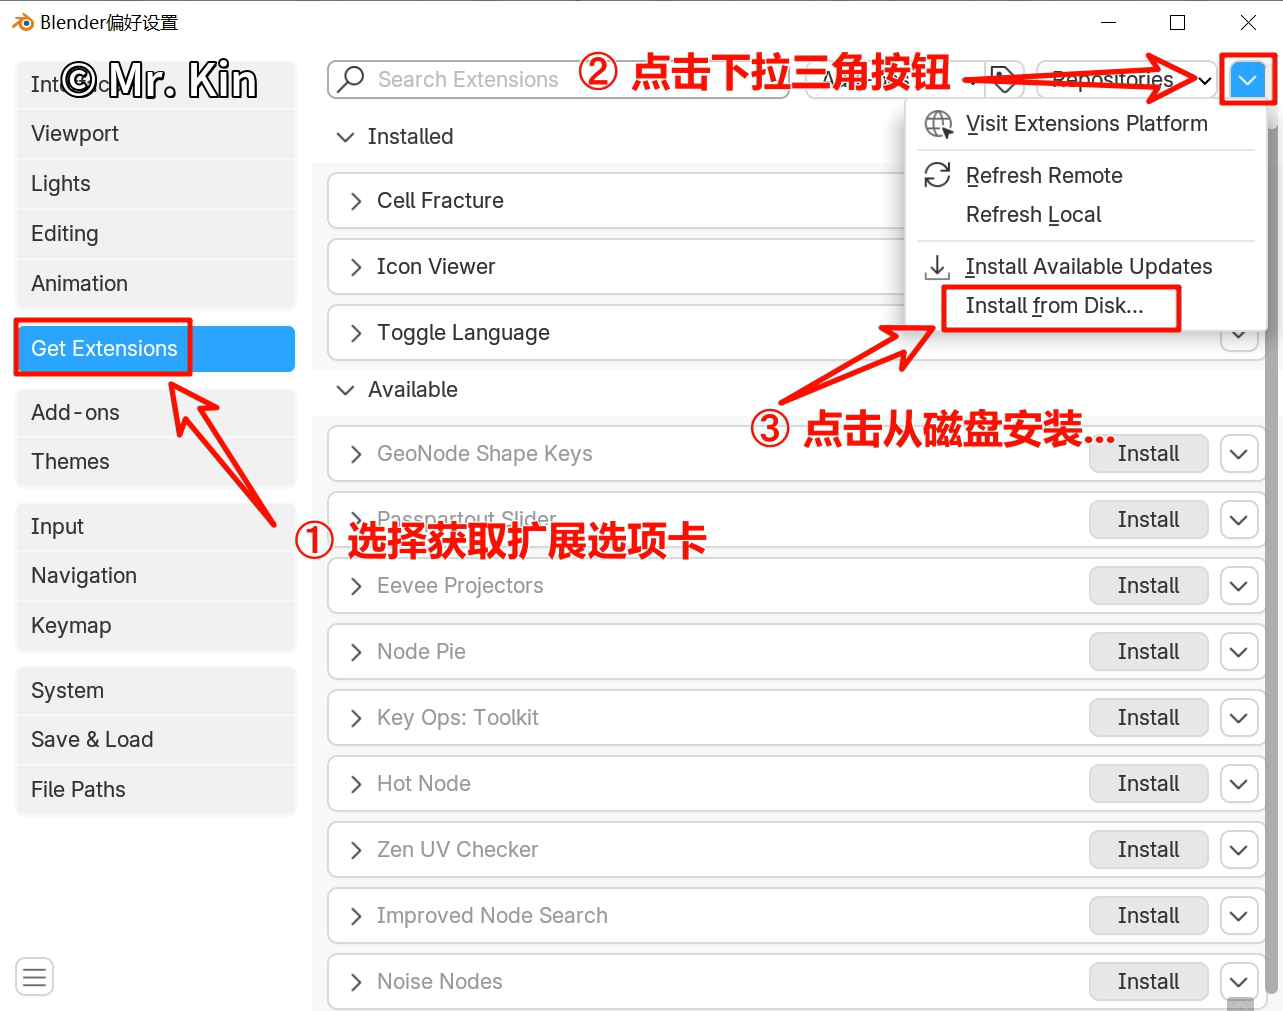
\includegraphics[width=\linewidth]{tab_get_extensions}
        \caption{获取扩展选项卡}
    \end{minipage}
    \quad
    \begin{minipage}[t]{0.48\linewidth}
        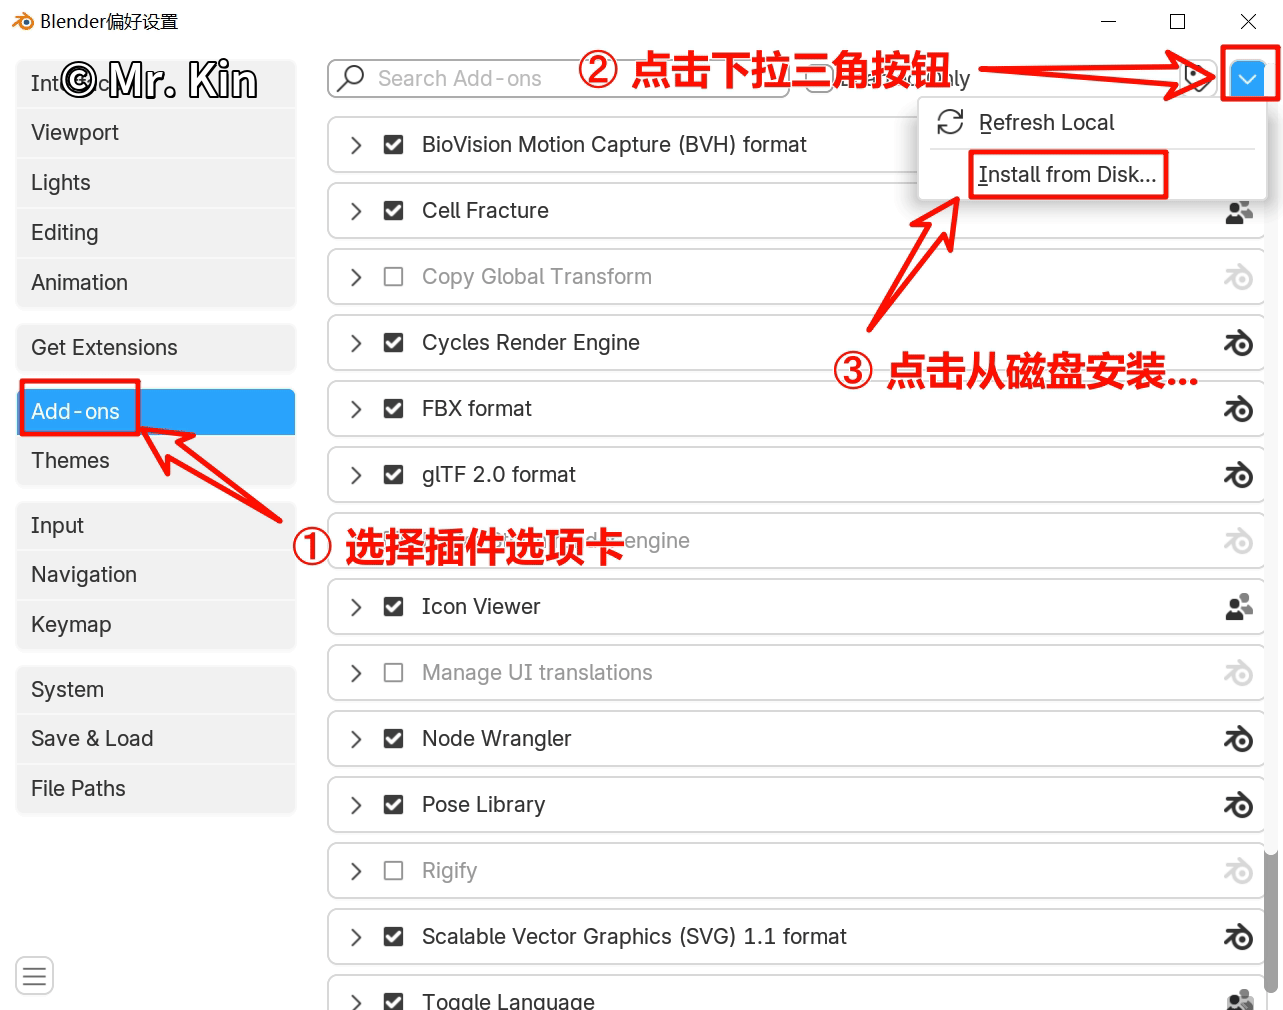
\includegraphics[width=\linewidth]{tab_addon}
        \caption{插件选项卡}
    \end{minipage}
\end{figure}

\subsubsection{在线安装}
\note{因「\href{https://extensions.blender.org/}{Blender Extension平台}」网站管理员认为本插件存在多项功能并不符合插件名称,管理员称这不符合规范,故本人已选择删除\href{https://id.blender.org/}{Blender ID}帐号。自2024-12-26起,不再支持插件以「官方在线扩展插件平台】方式来在线安装。—— Mr. Kin,2024-12-26}

\note{后续版本将会基于\href{https://github.com/Mister-Kin/ToggleLanguage/releases}{Github Rleases}开发实现支持自动检查版本和自动更新功能,敬请期待!—— Mr. Kin,2024-12-26}

\sout{blender v4.2之后版本(含v4.2)上线了extensions插件功能,允许从官方维护}
\noindent\sout{的扩展平台中直接安装扩展插件。本插件已上架官方扩展平台,可以直接搜索「toggle language」进行安装。}

\noindent (该步骤已不再支持!!!)安装步骤:
\begin{enumerate}
    \item 运行Blender。
    \item 打开「Preferences/用户偏好设置」(Menu/菜单 >Edit/编辑>Preferences/用户偏好设置)。
    \item 选择「Get Extensions/获取扩展」选项卡。
    \item 点击「Allow Online Access/允许在线访问」
    \item 搜索框内输入「toggle language」
    \item 点击「Install/安装」
\end{enumerate}

\begin{figure}[h!]
    \begin{minipage}[t]{0.48\linewidth}
        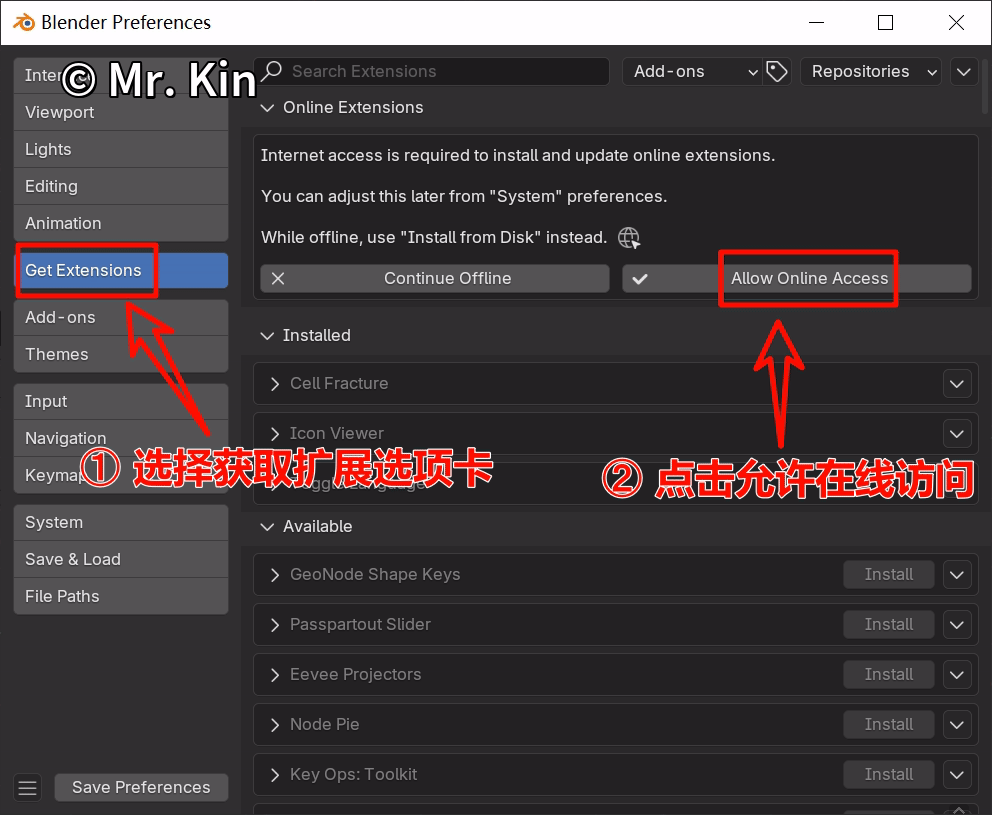
\includegraphics[width=\linewidth]{online_install_step12}
        \caption{在线安装步骤1\&2}
    \end{minipage}
    \quad
    \begin{minipage}[t]{0.48\linewidth}
        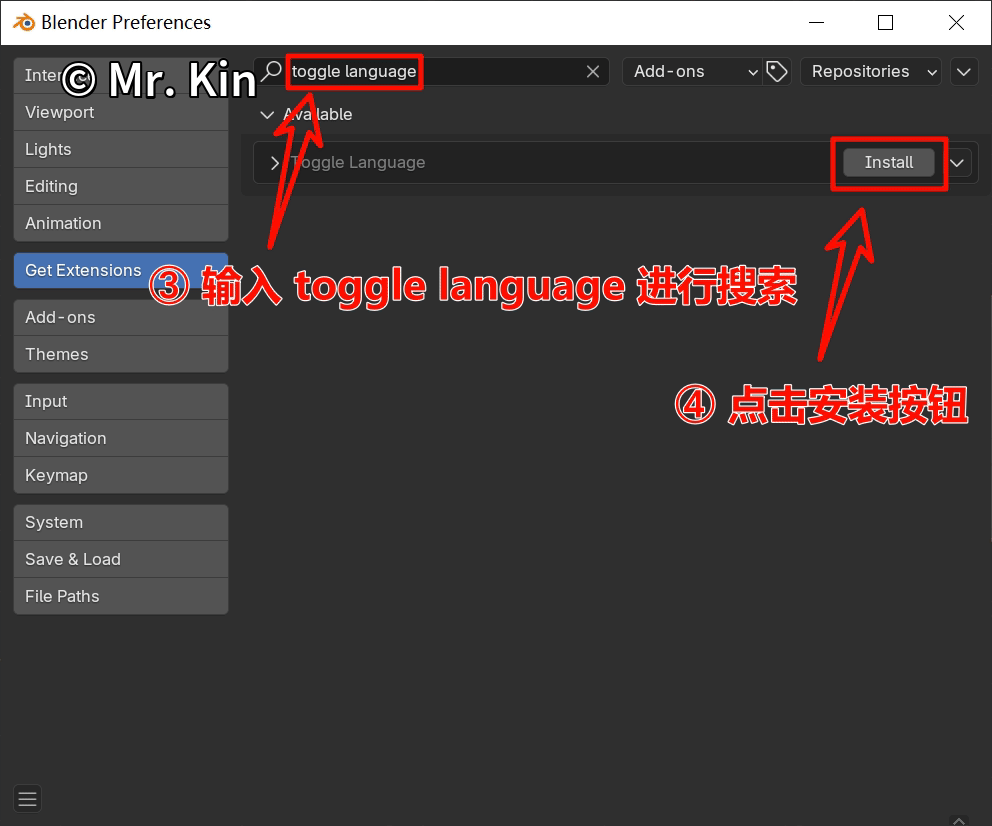
\includegraphics[width=\linewidth]{online_install_step34}
        \caption{在线安装步骤3\&4}
    \end{minipage}
\end{figure}

\subsection{下载及安装(v2.83-v4.1.1)}
\hypertarget{install_v283_v411}{}
\subsubsection{下载步骤}
\begin{itemize}
    \item 插件下载链接:\href{https://github.com/Mister-Kin/ToggleLanguage/releases/latest}{Github Release},在\lstinline|Assets|资产中下载 ToggleLanguage.zip 文件。
    \item blender版本要求:\href{https://www.blender.org/download/}{v2.83+}
\end{itemize}
\note{blender v2.83默认是启用翻译功能,这也是本插件要求将v2.83作为最低版本的缘由。本插件也许在v2.83以下版本能够运行,但不推荐,因为没测试过。}

\subsubsection{安装步骤}
\begin{enumerate}
    \item 运行Blender。
    \item 打开「Preferences/用户偏好设置」(Menu/菜单>Edit/编辑>Preferences/用户偏好设置)。
    \item 选择「Add-ons/插件」选项卡。
    \item 点击「Install.../安装」后,选择先前所下载好的ToggleLanguage.zip并点击确定。
    \item 启用插件。
\end{enumerate}

\begin{figure}[h!]
    \begin{minipage}[t]{0.48\linewidth}
        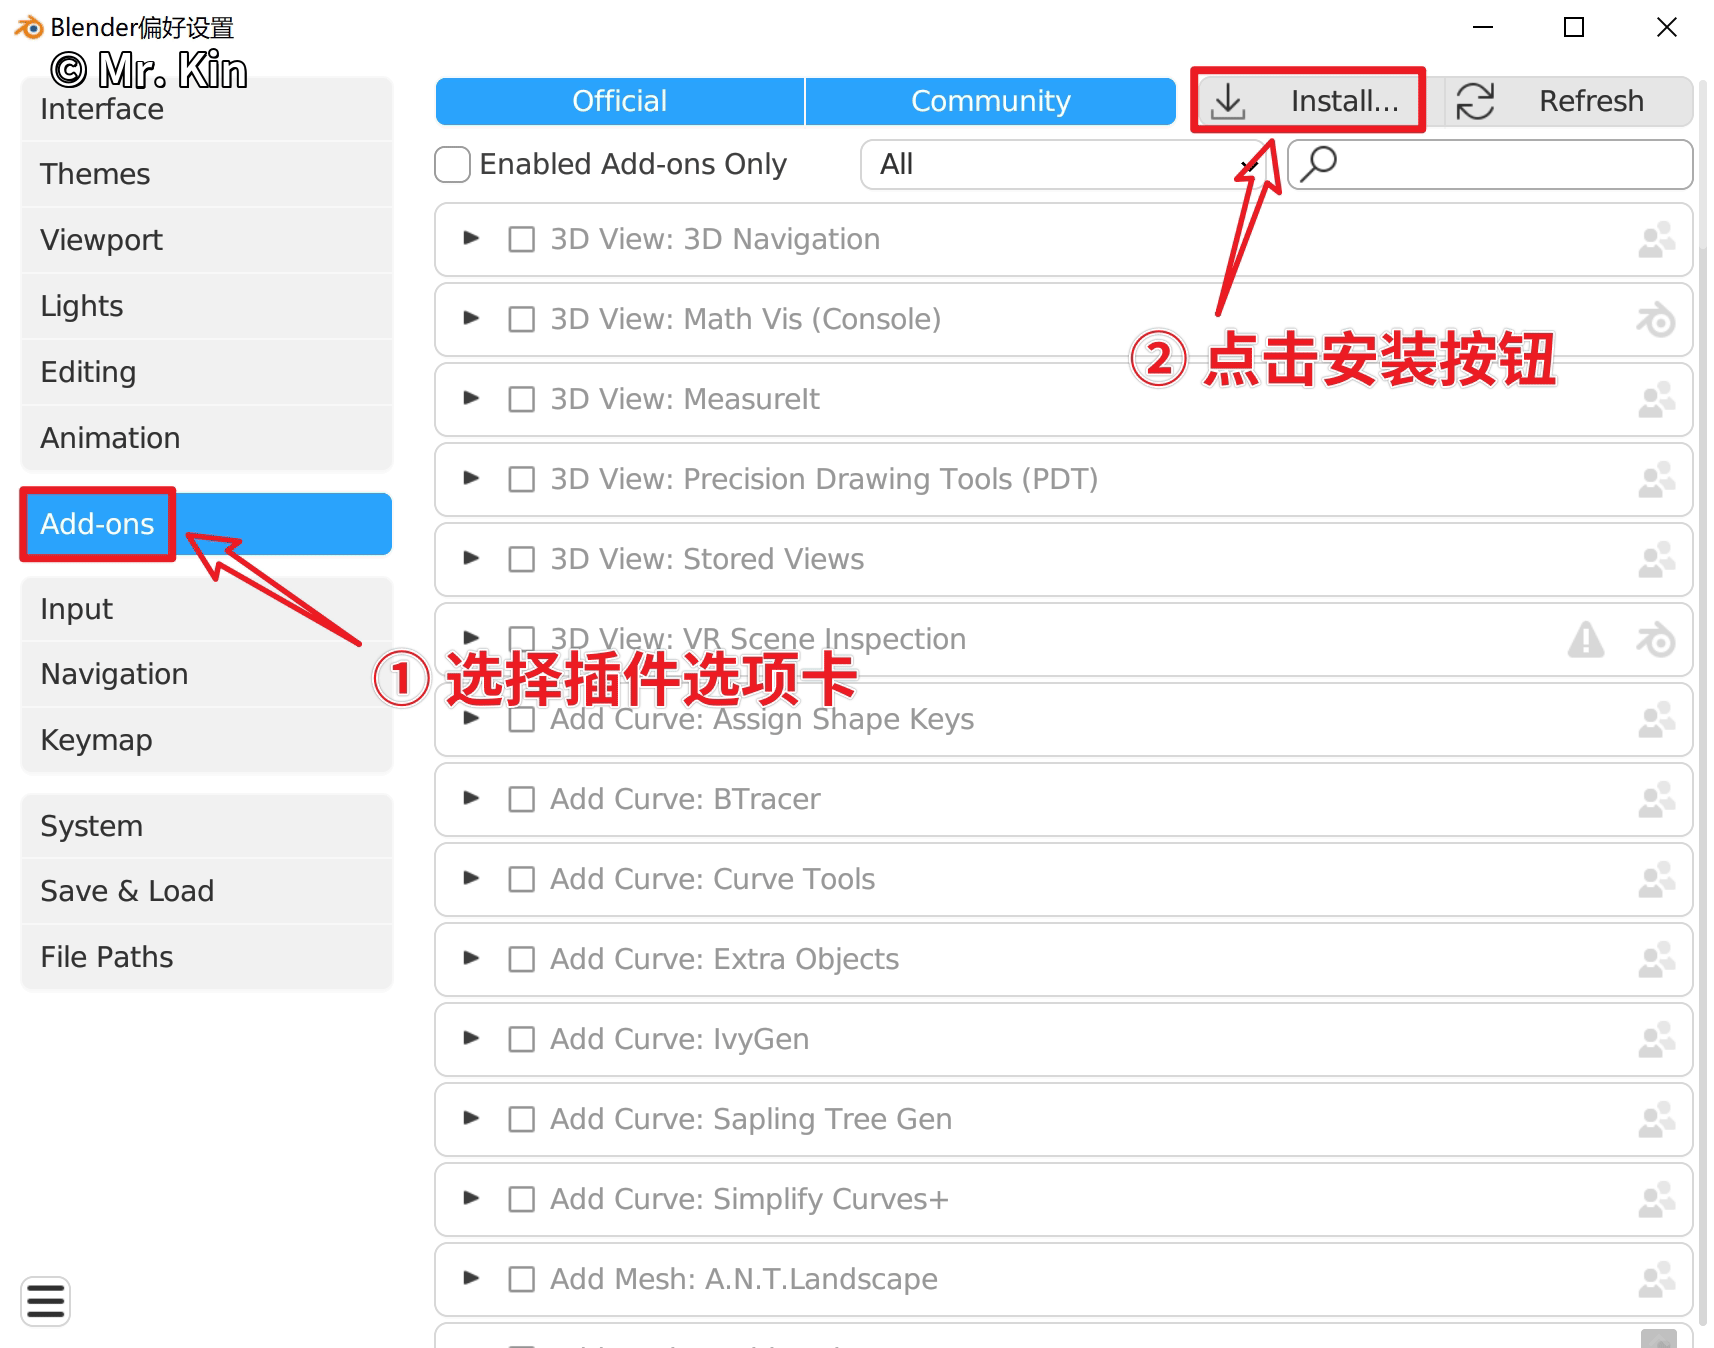
\includegraphics[width=\linewidth]{installation}
        \caption{安装方法}
    \end{minipage}
    \quad
    \begin{minipage}[t]{0.48\linewidth}
        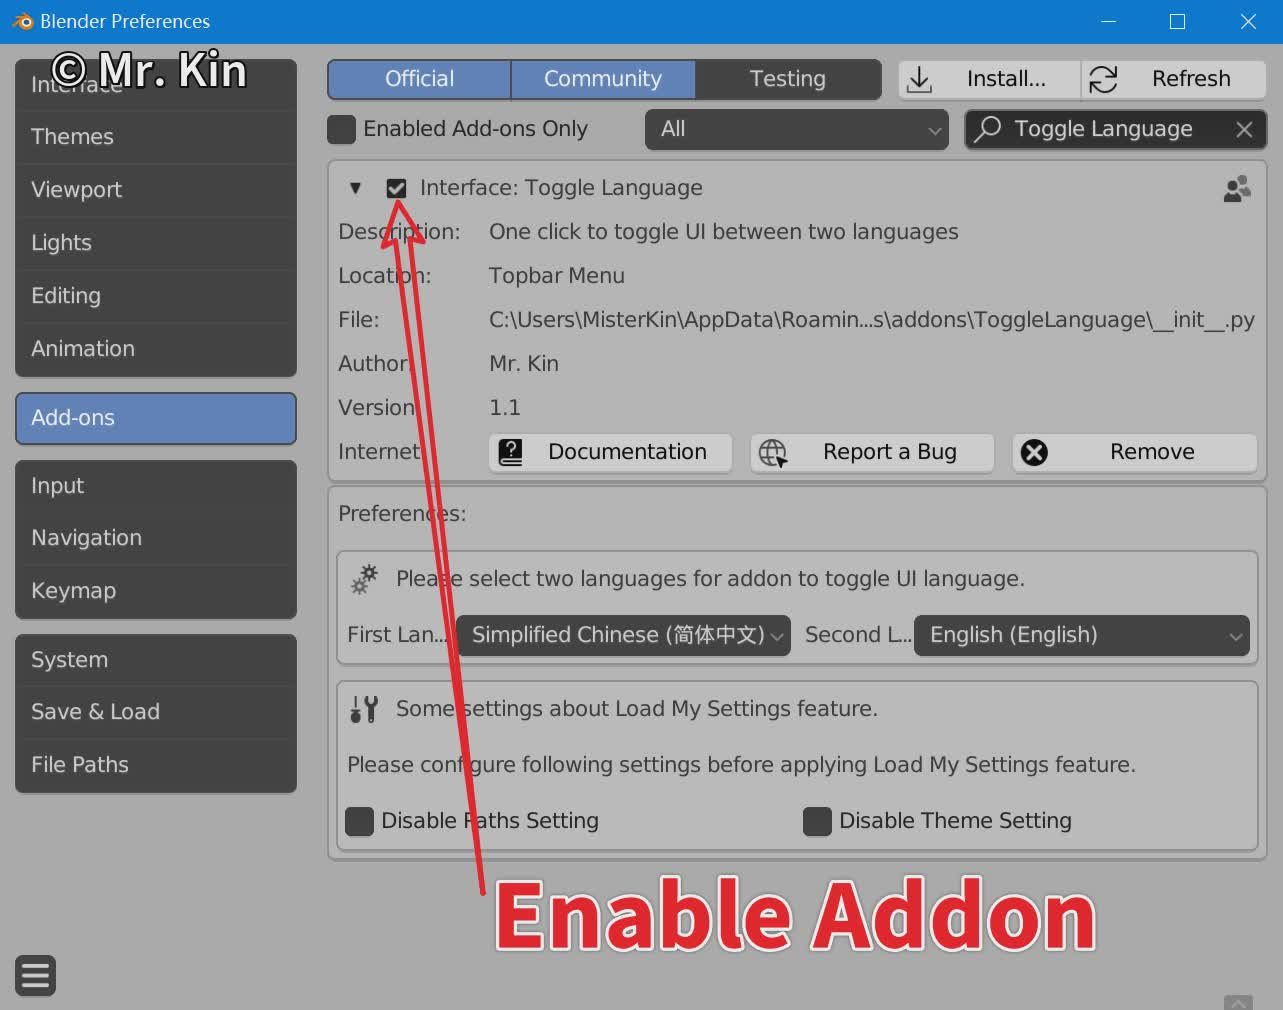
\includegraphics[width=\linewidth]{enable_addon}
        \caption{启用插件}
        \label{启用插件}
    \end{minipage}
\end{figure}

\subsection{插件UI}
\label{插件UI小节}
如图\myref{插件UI}所示,启用插件后,可看见插件位于顶部菜单栏末尾处。插件UI从左往右看,有四个元素:
\begin{enumerate}
    \item 语言切换按钮
    \item 实用工具菜单
    \item 插件的个性化设置菜单
    \item 用户偏好设置按钮
\end{enumerate}

\begin{figure}[h!]
    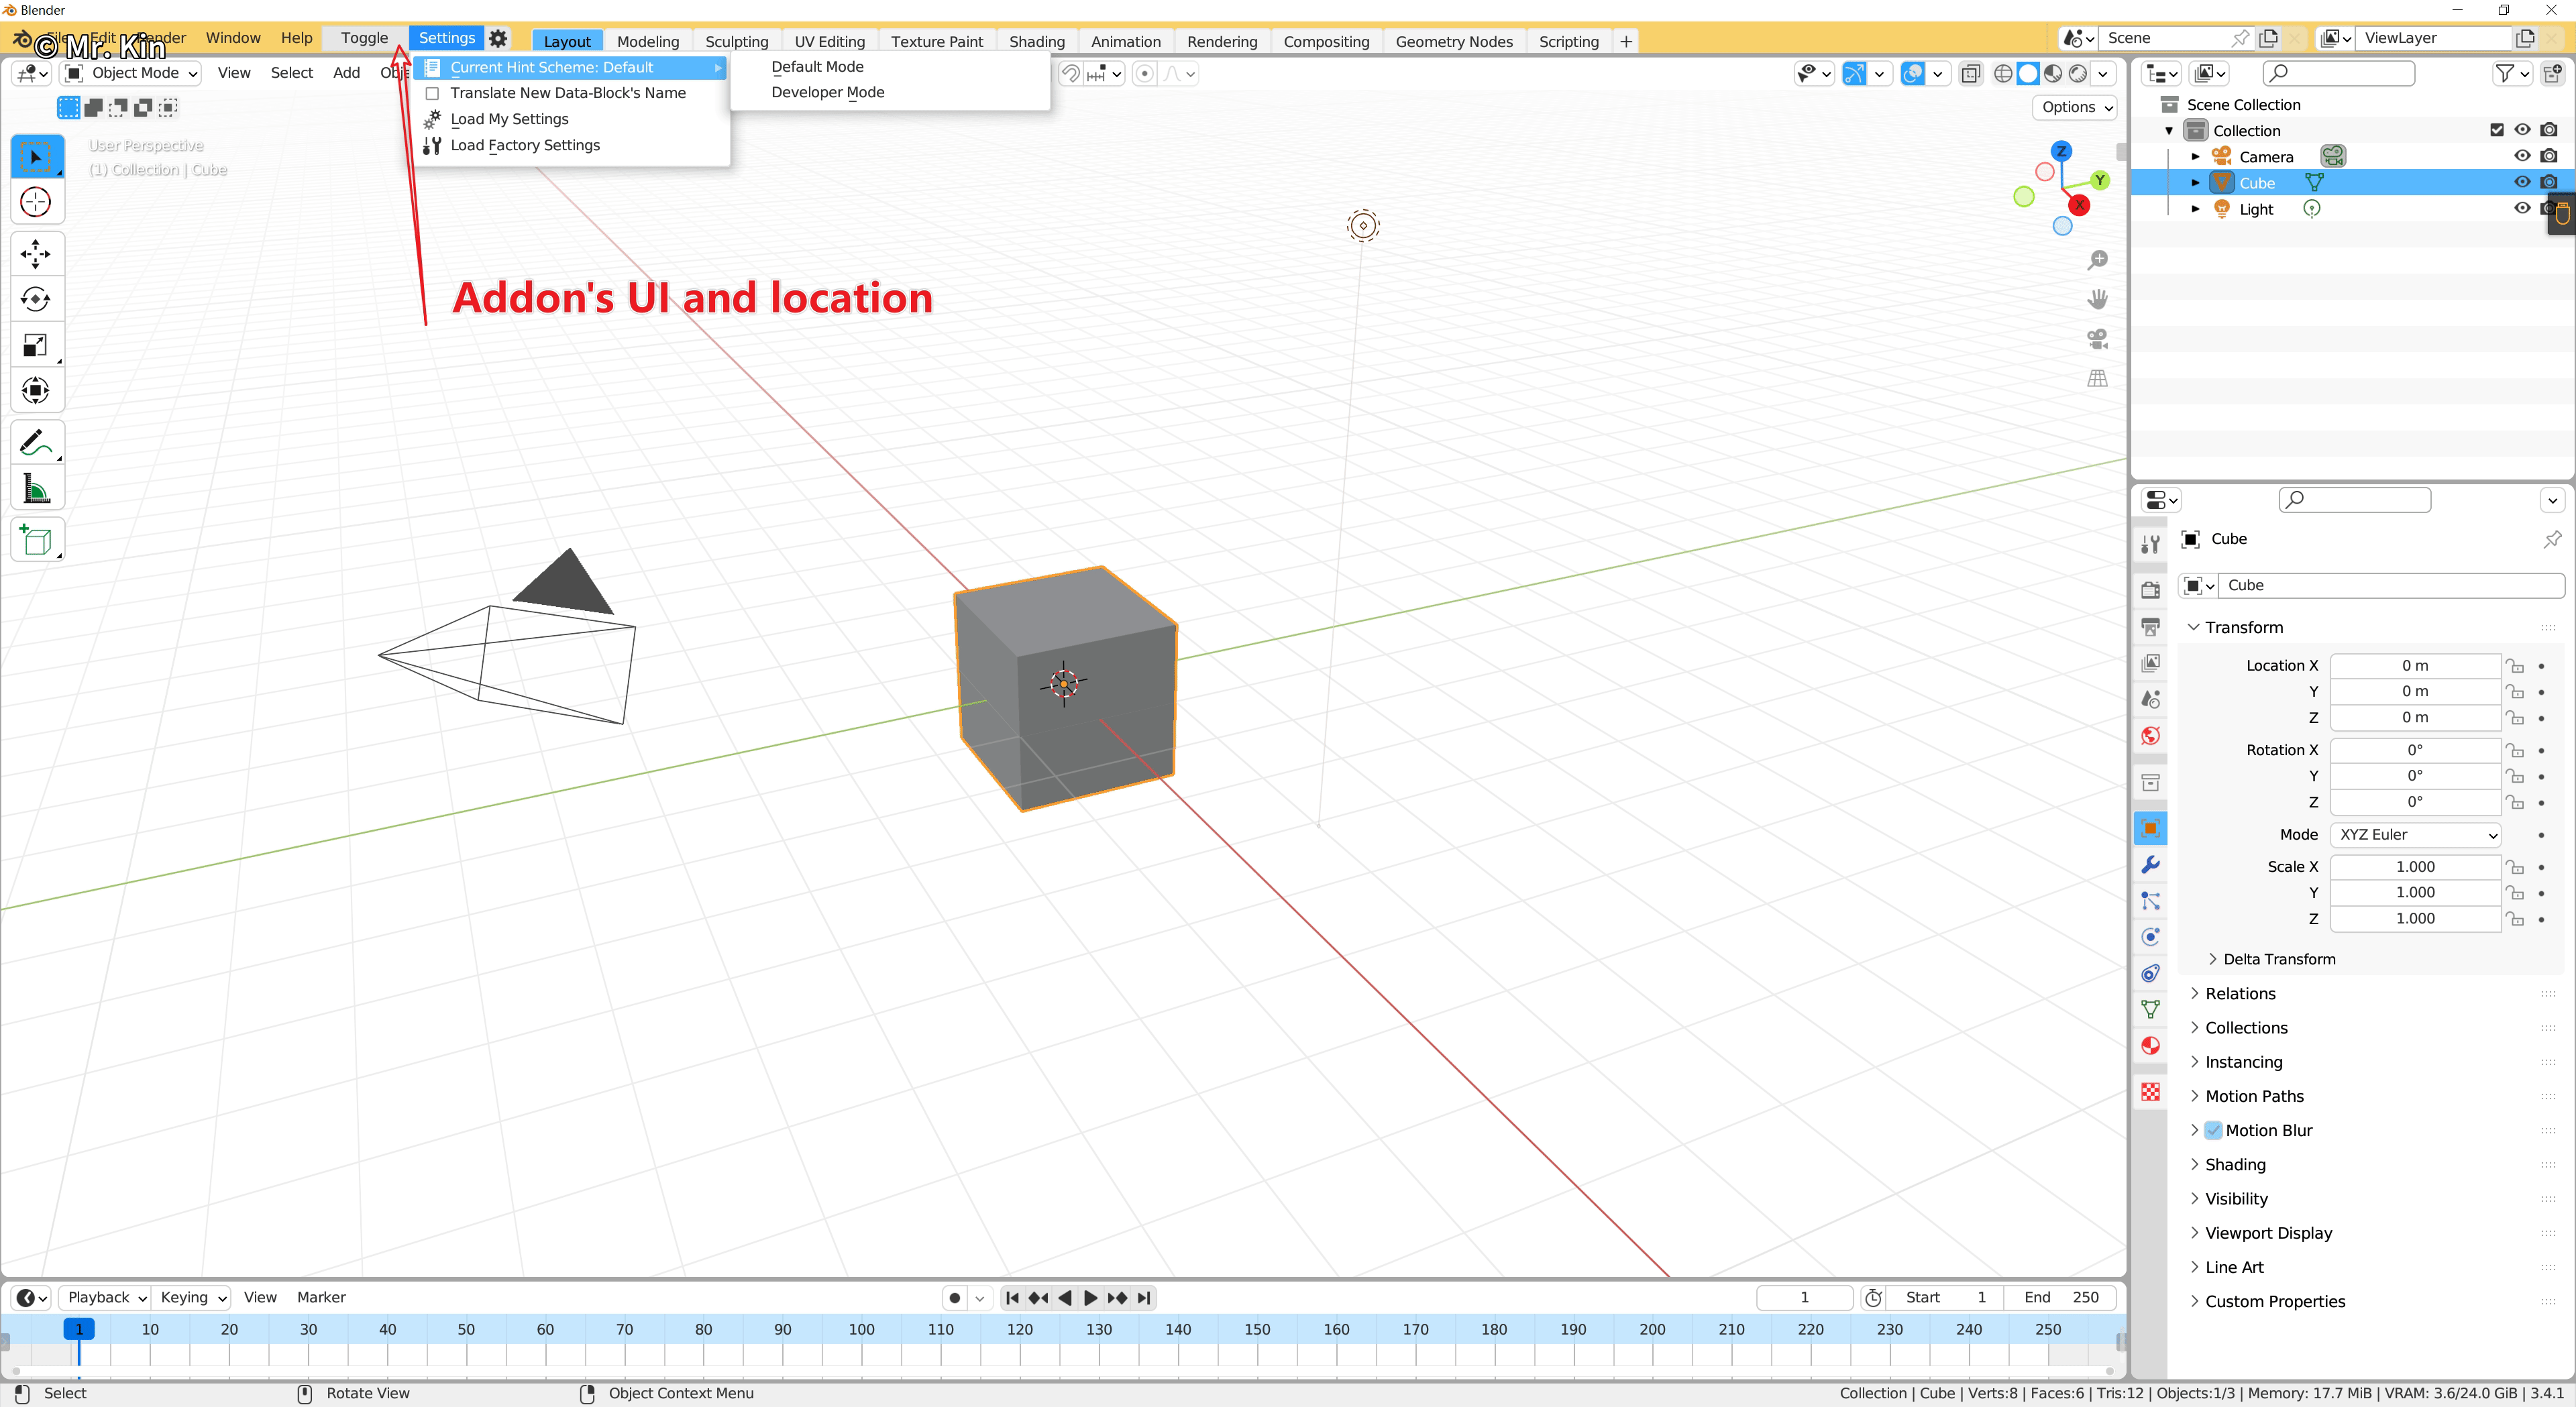
\includegraphics[width=\linewidth]{ui}
    \caption{插件UI}
    \label{插件UI}
\end{figure}

\subsection{插件功能}
\hypertarget{AddonFeatures}{}

\note{以下按照UI排列位置进行功能介绍。UI排列位置详见「\nameref{插件UI小节}」小节。}

\begin{enumerate}
    \item 语言切换按钮(快捷键F5):在两种语言之间切换blender用户界面语言(支持多种语言相互切换)。插件允许自定义该快捷键,详见「\hyperlink{AddonKeymaps}{插件的键位映射}」小节内容。
    \item 实用工具菜单:一些实用工具集合
    \begin{enumerate}
        \item 删除当前场景中所有集合和物体:清空场景,即删除当前场景中的所有集合和物体。
        \item 添加视频进度条:在VSE的频道顶部空白区域添加视频进度条,如图\myref{视频进度条复合片段}和图\myref{视频进度条子片段}所示。视频进度条为一个复合片段,相关参数为:置于视频顶部,高度44px,透明度0.9,底部进度条颜色RGB(0.45, 0.45, 0.45),滚动进度条颜色RGB(0.255, 0.255, 0.255)。P.S. 后续会开发增设一个调整视频进度条参数的窗口。
    \end{enumerate}
    \item 设置菜单:插件的个性化设置。
    \begin{enumerate}
        \item UI提示方案菜单:选择相应UI提示的方案。
        \begin{enumerate}
            \item 默认模式:禁用「开发选项」「Python工具提示」,如图\myref{默认提示方案}所示。
            \item 开发者模式:启用「开发选项」「Python工具提示」,如图\myref{开发者提示方案}所示。
        \end{enumerate}
        \item 翻译新建数据块的名称按钮:启用/禁用新建数据块名称的翻译功能\footnote{v1.1之后版本不再是强制接管该功能。虽然可以通过用户偏好设置来设置一个不同于插件的设置值,但在使用插件的该功能或者语言切换按钮后,插件会对该项改写修正为插件的设置值。},默认值为禁用,如图\myref{插件的翻译名称选项}所示,其对应在偏好设置中的选项如图\myref{偏好设置的的翻译名称选项}所示。在非英语界面环境中,启用该功能可使blender新建数据块的名称为当前语言,如图\myref{翻译名称的效果}所示,新建平面的名称为「平面」,而非「plane」。
        \item 加载我的Blender设置按钮:部署我个人的偏好设置。所涉及的设置选项详见\hyperlink{MySettings}{我的设置}。该功能默认会覆盖你原有的blender设置(启动文件和偏好设置),请详细了解所涉及的设置项后再确认是否使用该功能。\footnote{理论上支持任意系统、任意安装路径、任意显卡平台的情况,但Linux OS和Mac OS比较少测试,可能会存在有bug。}
        \item 加载Blender初始设置按钮:加载初始的偏好设置和启动文件,即重置blender,还原成初次安装blender时的状态。
    \end{enumerate}
    \item 用户偏好设置按钮(快捷键Ctrl+Alt+U):打开用户偏好设置窗口。插件允许自定义该快捷键,详见「\hyperlink{AddonKeymaps}{插件的键位映射}」小节内容。
\end{enumerate}

\subsubsection{插件切换语言的设置}
在本插件的偏好设置面板中,可以设置切换语言功能所需的语言项,如图\myref{启用插件}所示,两个语言项的默认值分别为简体中文和英语。两个语言项不分前后顺序,只要设置好两种不同语言,插件便可以在这两种语言之间切换UI界面。

本插件在blender v4.0以后(含blender v4.0)支持 18 种语言\footnote{即blender v4.0以后(含blender v4.0)内置翻译语言列表中Complete和In Progress两个列表中的语言,共18种。暂不考虑加入Starting列表中的语言,因为其变动性较高,有可能被删除或者新添加。}相互切换,详见下表:

\begin{itemize}
    \item Simplified Chinese (简体中文)
    \item Traditional Chinese (繁體中文)
    \item English (English)
    \item Catalan (Català)
    \item Spanish (Español)
    \item French (Français)
    \item Japanese (日本語)
    \item Slovak (Slovenčina)
    \item Czech (Čeština)
    \item German (Deutsch)
    \item Italian (Italiano)
    \item Georgian (ქართული)
    \item Korean (한국어)
    \item Brazilian Portuguese (Português do Brasil)
    \item Portuguese (Português)
    \item Russian (Русский)
    \item Ukrainian (Українська)
    \item Vietnamese (Tiếng Việt)
\end{itemize}

目前本插件在blender v4.0以前(不含blender v4.0)支持 17 种语言\footnote{即blender v4.0以前(不含blender v4.0)内置翻译语言列表中Complete和In Progress两个列表中的语言,共17种。暂不考虑加入Starting列表中的语言,因为其变动性较高,有可能被删除或者新添加。}相互切换,详见下表:

\begin{itemize}
    \item Simplified Chinese (简体中文)
    \item Traditional Chinese (繁體中文)
    \item English (English)
    \item Spanish (Español)
    \item Japanese (日本語)
    \item Slovak (Slovenčina)
    \item Ukrainian (Український)
    \item Vietnamese (tiếng Việt)
    \item Arabic (ﺔﻴﺑﺮﻌﻟﺍ)
    \item Czech (Český)
    \item German (Deutsch)
    \item French (Français)
    \item Italian (Italiano)
    \item Korean (한국 언어)
    \item Brazilian Portuguese (Português do Brasil)
    \item Portuguese (Português)
    \item Russian (Русский)
\end{itemize}

\begin{figure}[h!]
    \begin{minipage}[t]{0.48\linewidth}
        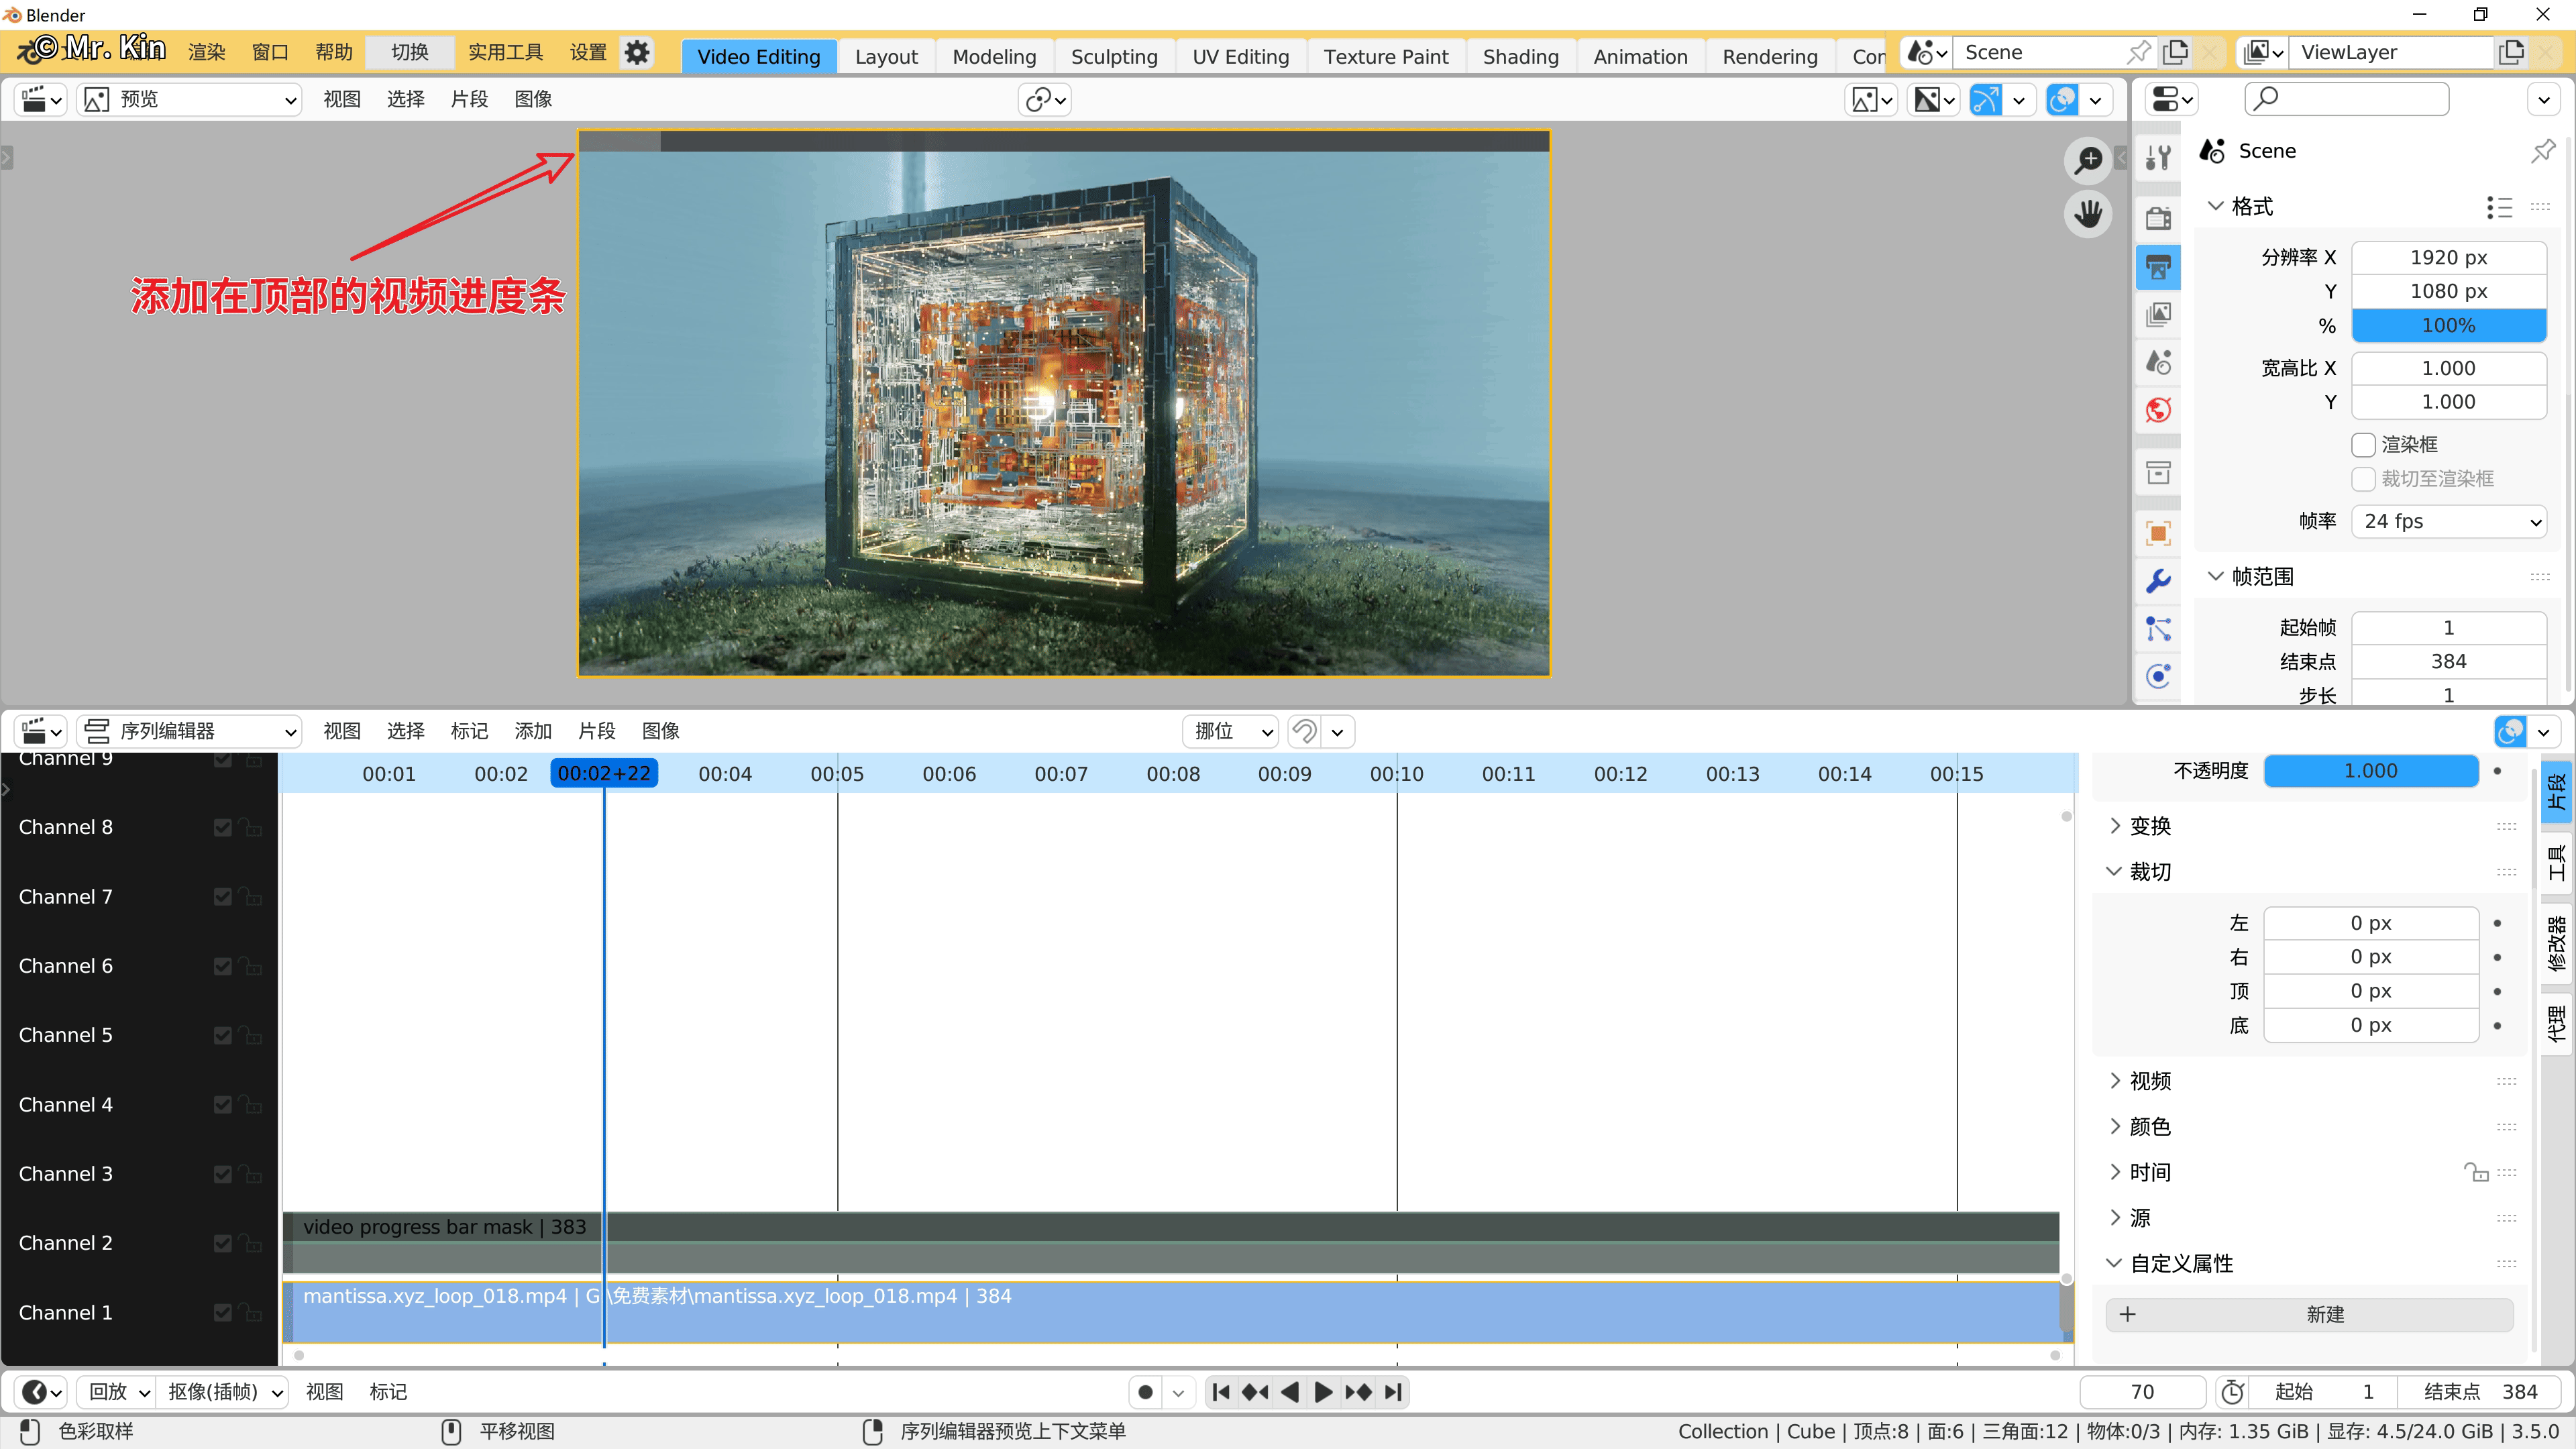
\includegraphics[width=\linewidth]{video_progress_bar_meta_strip}
        \caption{视频进度条 - 复合片段}
        \label{视频进度条复合片段}
    \end{minipage}
    \quad
    \begin{minipage}[t]{0.48\linewidth}
        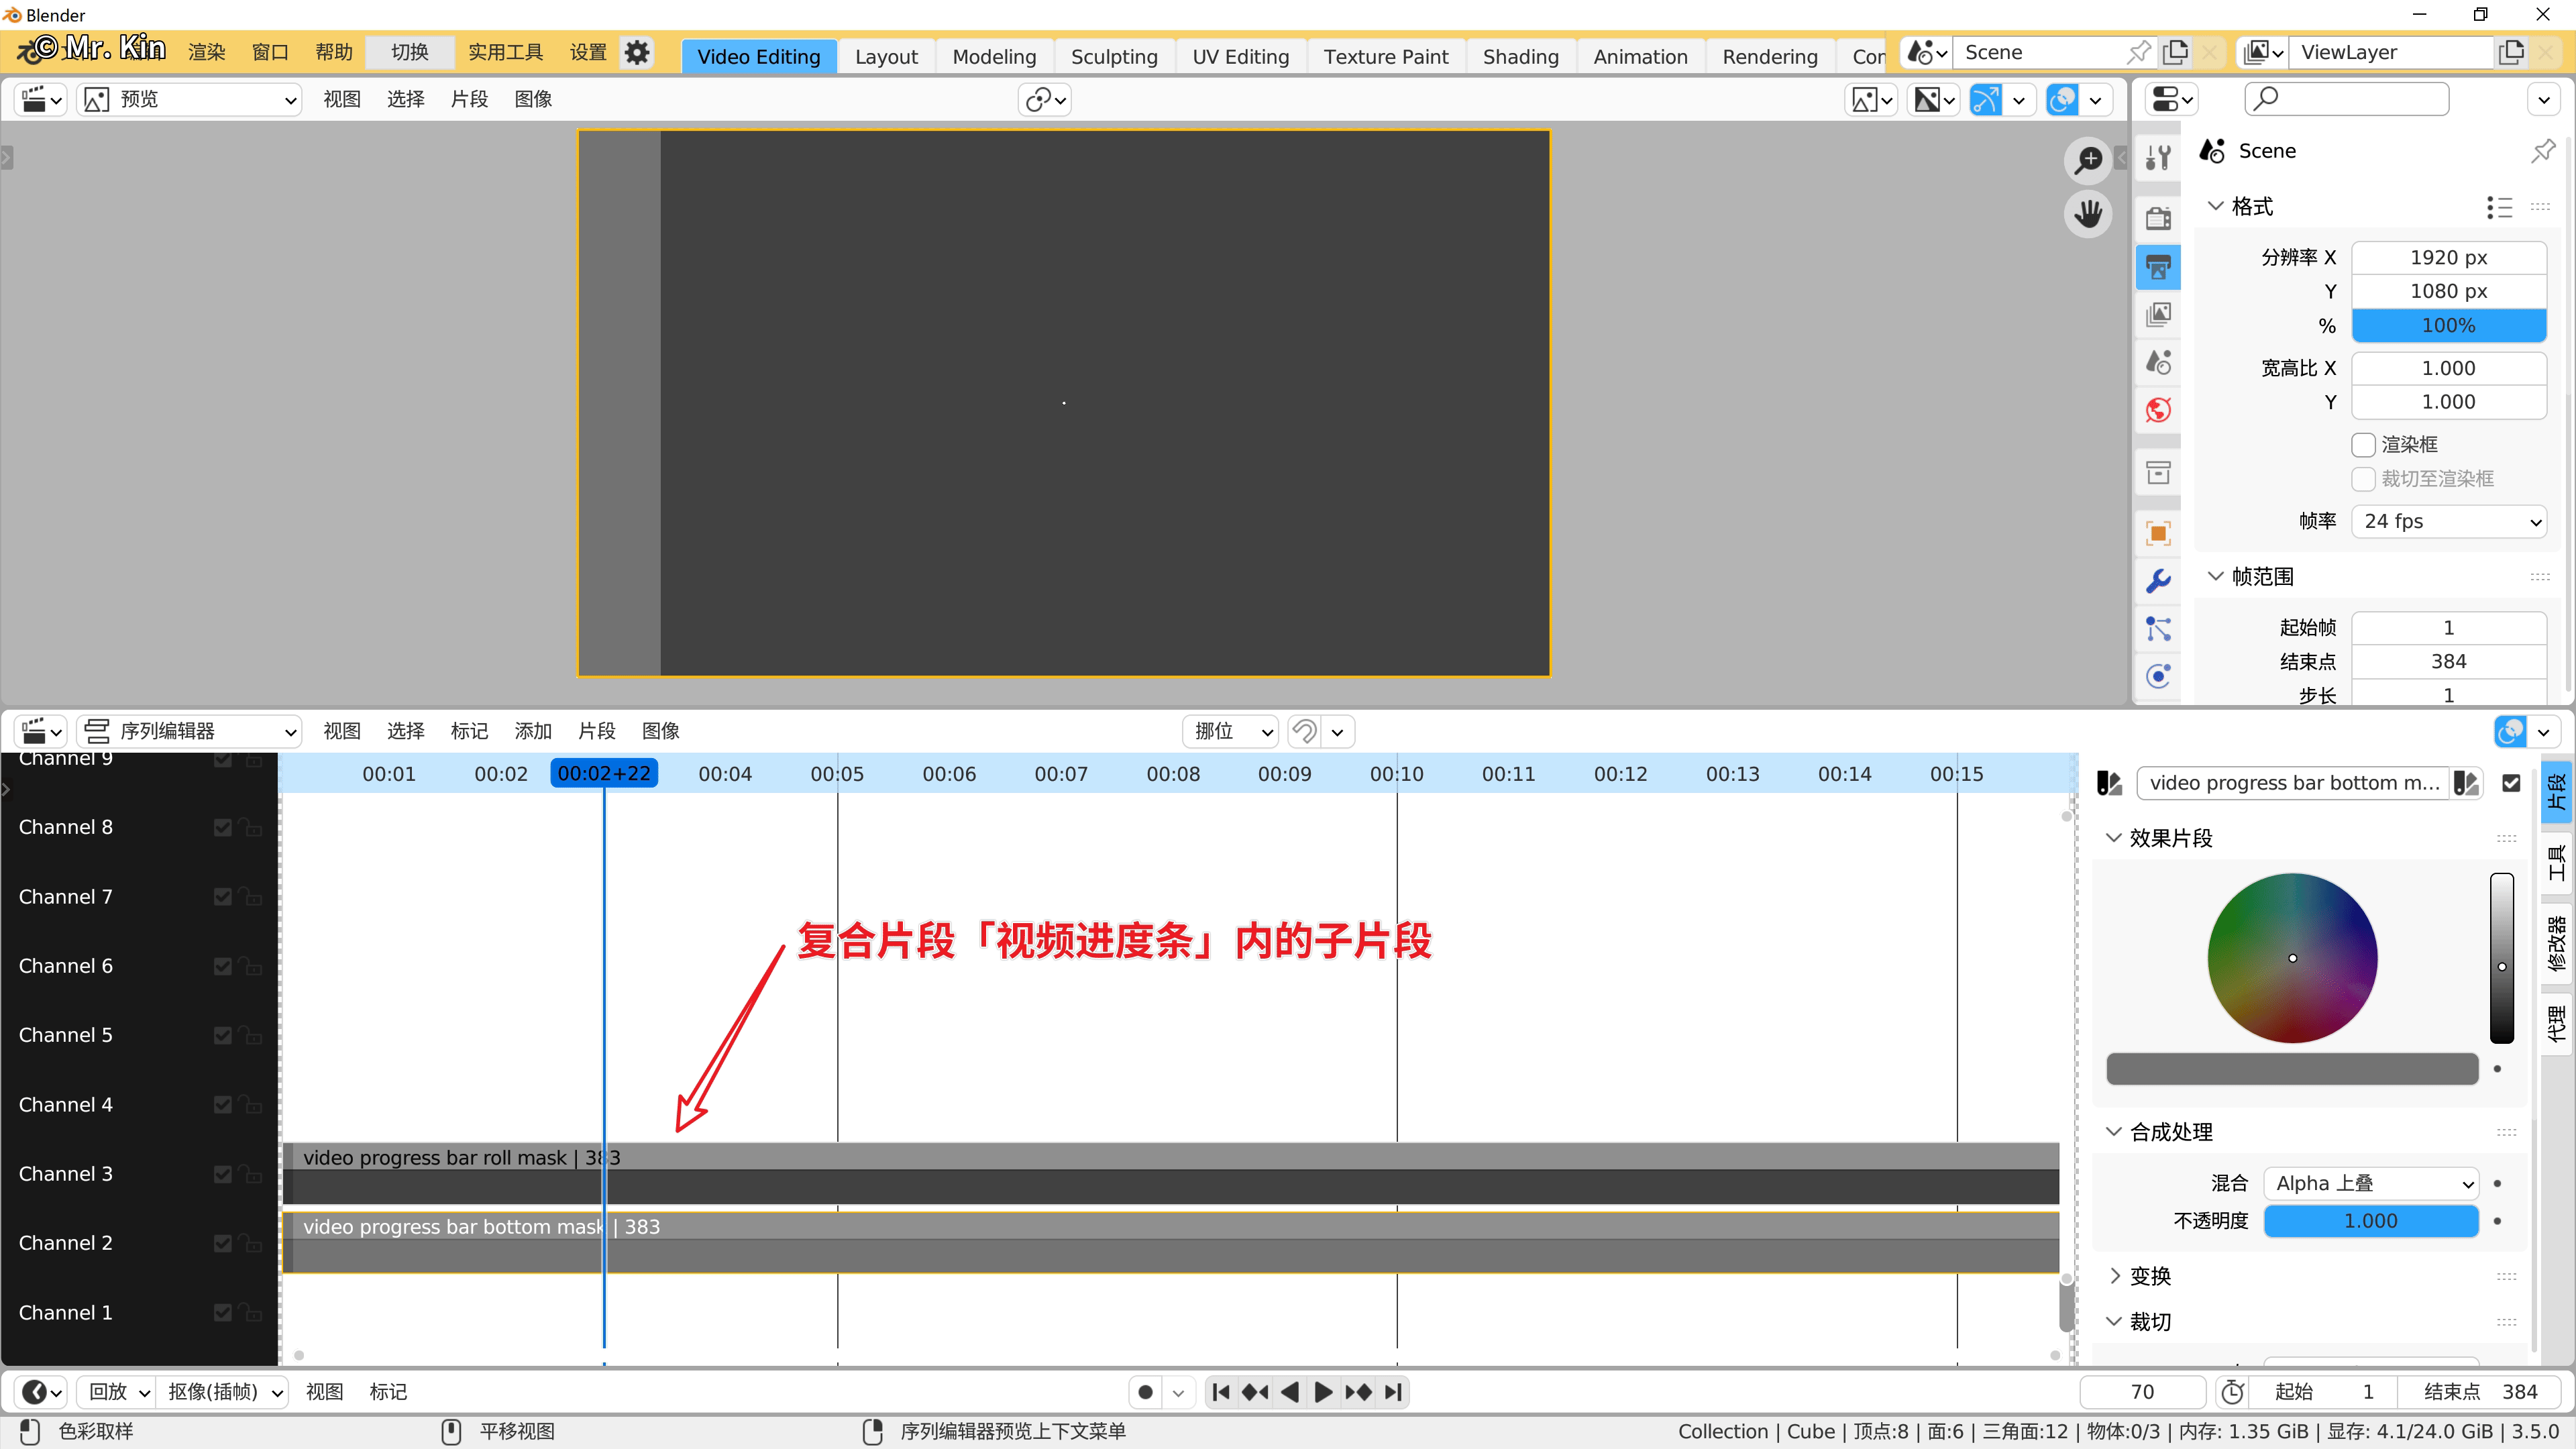
\includegraphics[width=\linewidth]{video_progress_bar_child_strip}
        \caption{复合片段「视频进度条」内的子片段}
        \label{视频进度条子片段}
    \end{minipage}

    \vspace{1ex}

    \begin{minipage}[t]{0.48\linewidth}
        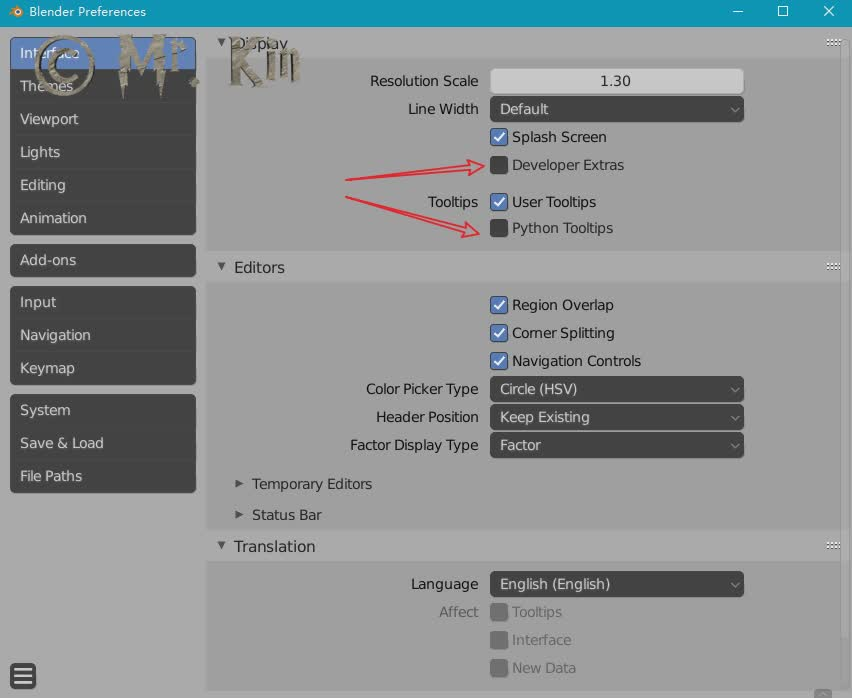
\includegraphics[width=\linewidth]{default_hint}
        \caption{UI提示方案菜单:默认模式}
        \label{默认提示方案}
    \end{minipage}
    \quad
    \begin{minipage}[t]{0.48\linewidth}
        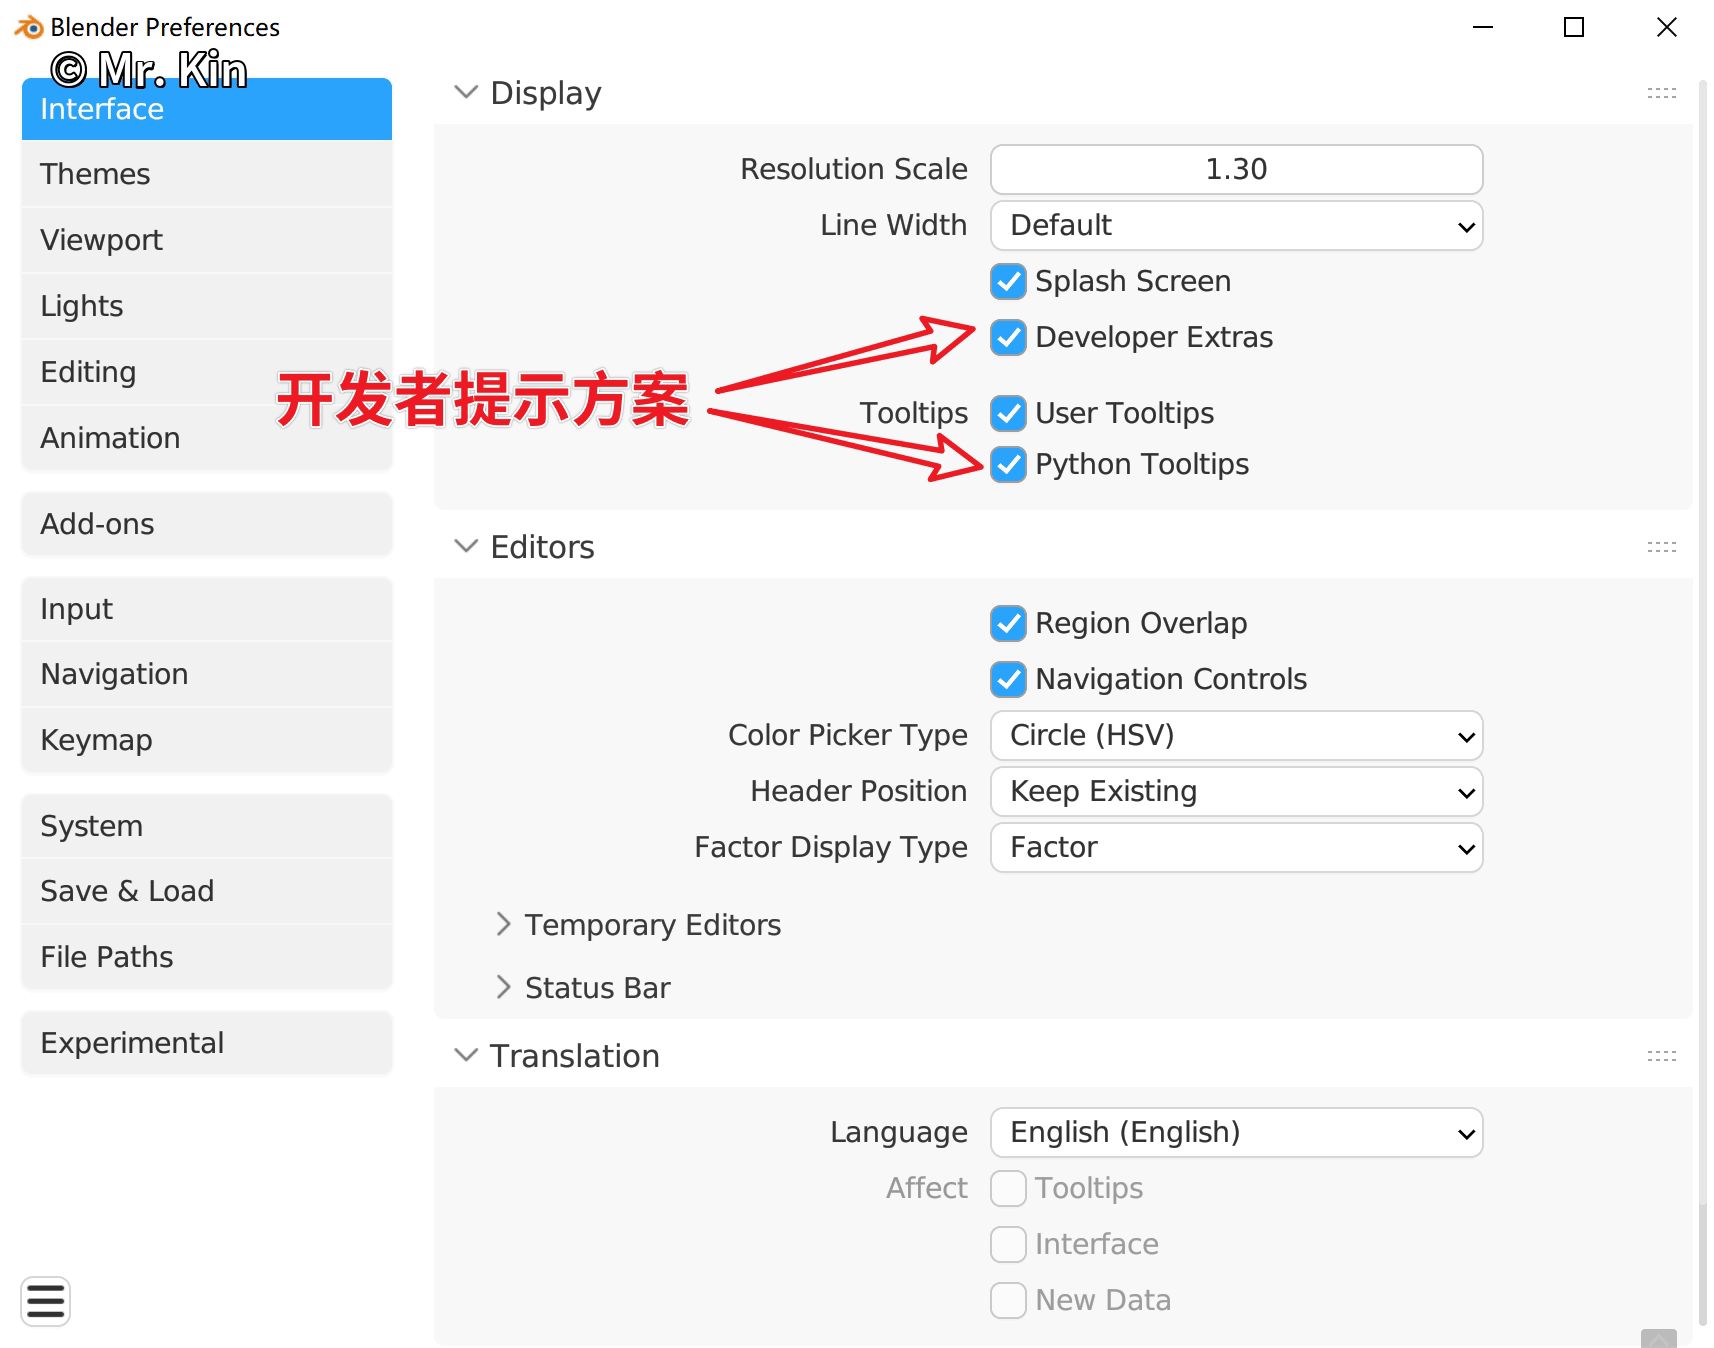
\includegraphics[width=\linewidth]{developer_hint}
        \caption{UI提示方案菜单:开发者模式}
        \label{开发者提示方案}
    \end{minipage}

    \vspace{1ex}

    \begin{minipage}[t]{0.45\linewidth}
        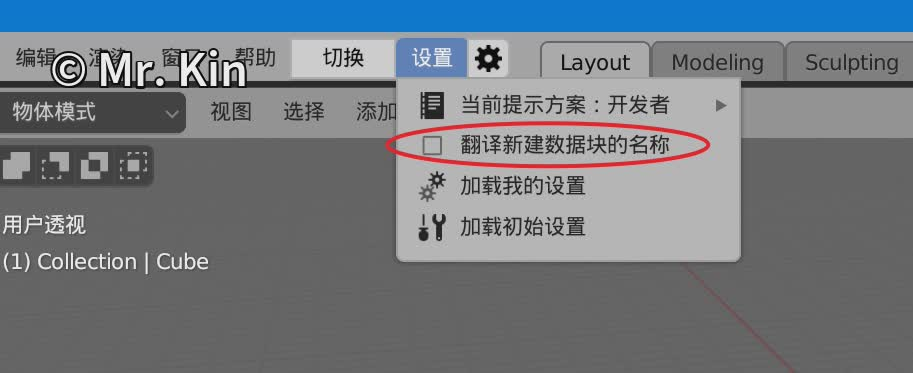
\includegraphics[width=\linewidth]{translate_name_option_addon}
        \caption{插件中的翻译新建数据块名称的选项}
        \label{插件的翻译名称选项}
    \end{minipage}
    \quad
    \begin{minipage}[t]{0.5\linewidth}
        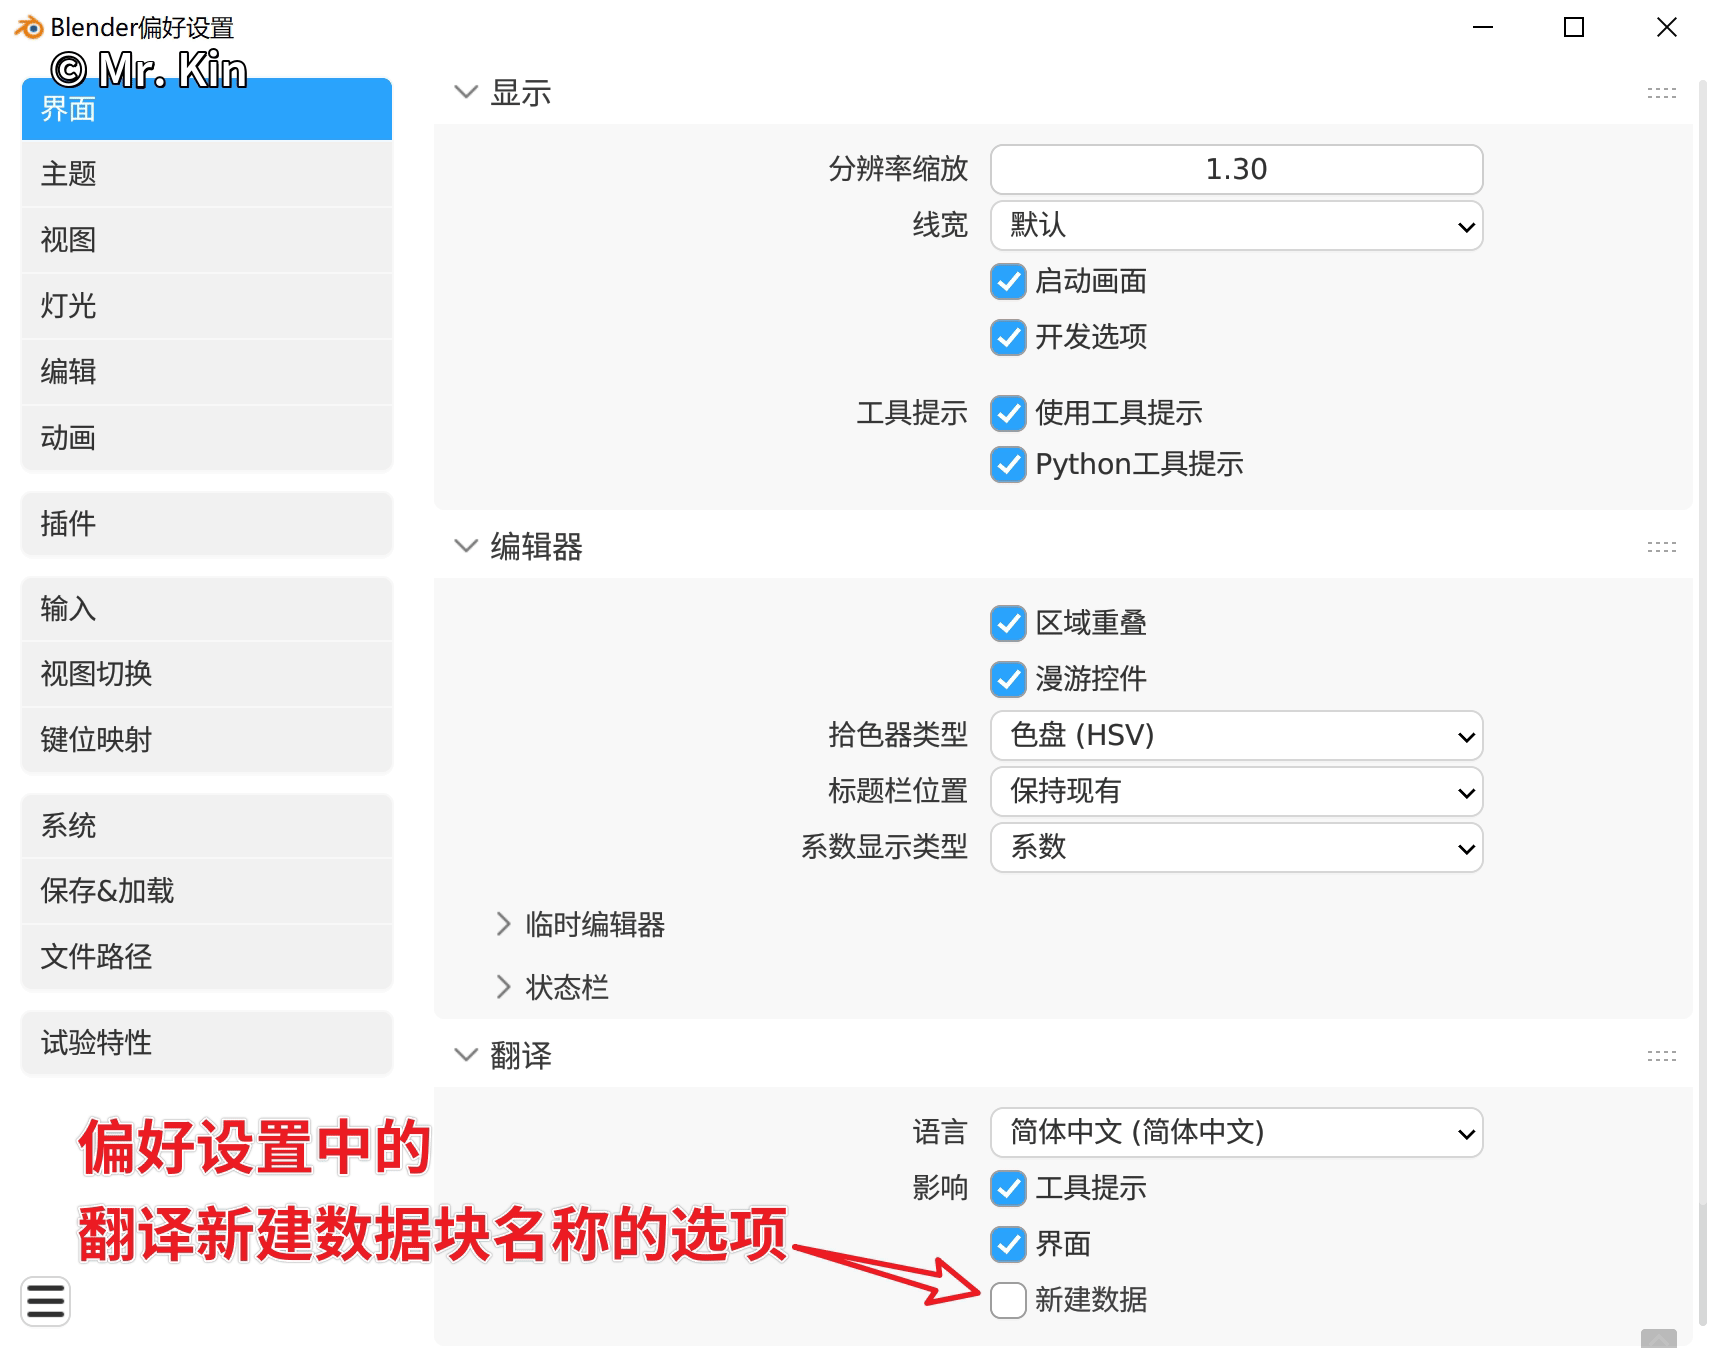
\includegraphics[width=\linewidth]{translate_name_option_pref}
        \caption{偏好设置中的翻译新建数据块名称的选项}
        \label{偏好设置的的翻译名称选项}
    \end{minipage}
\end{figure}

\clearpage

\begin{figure}
    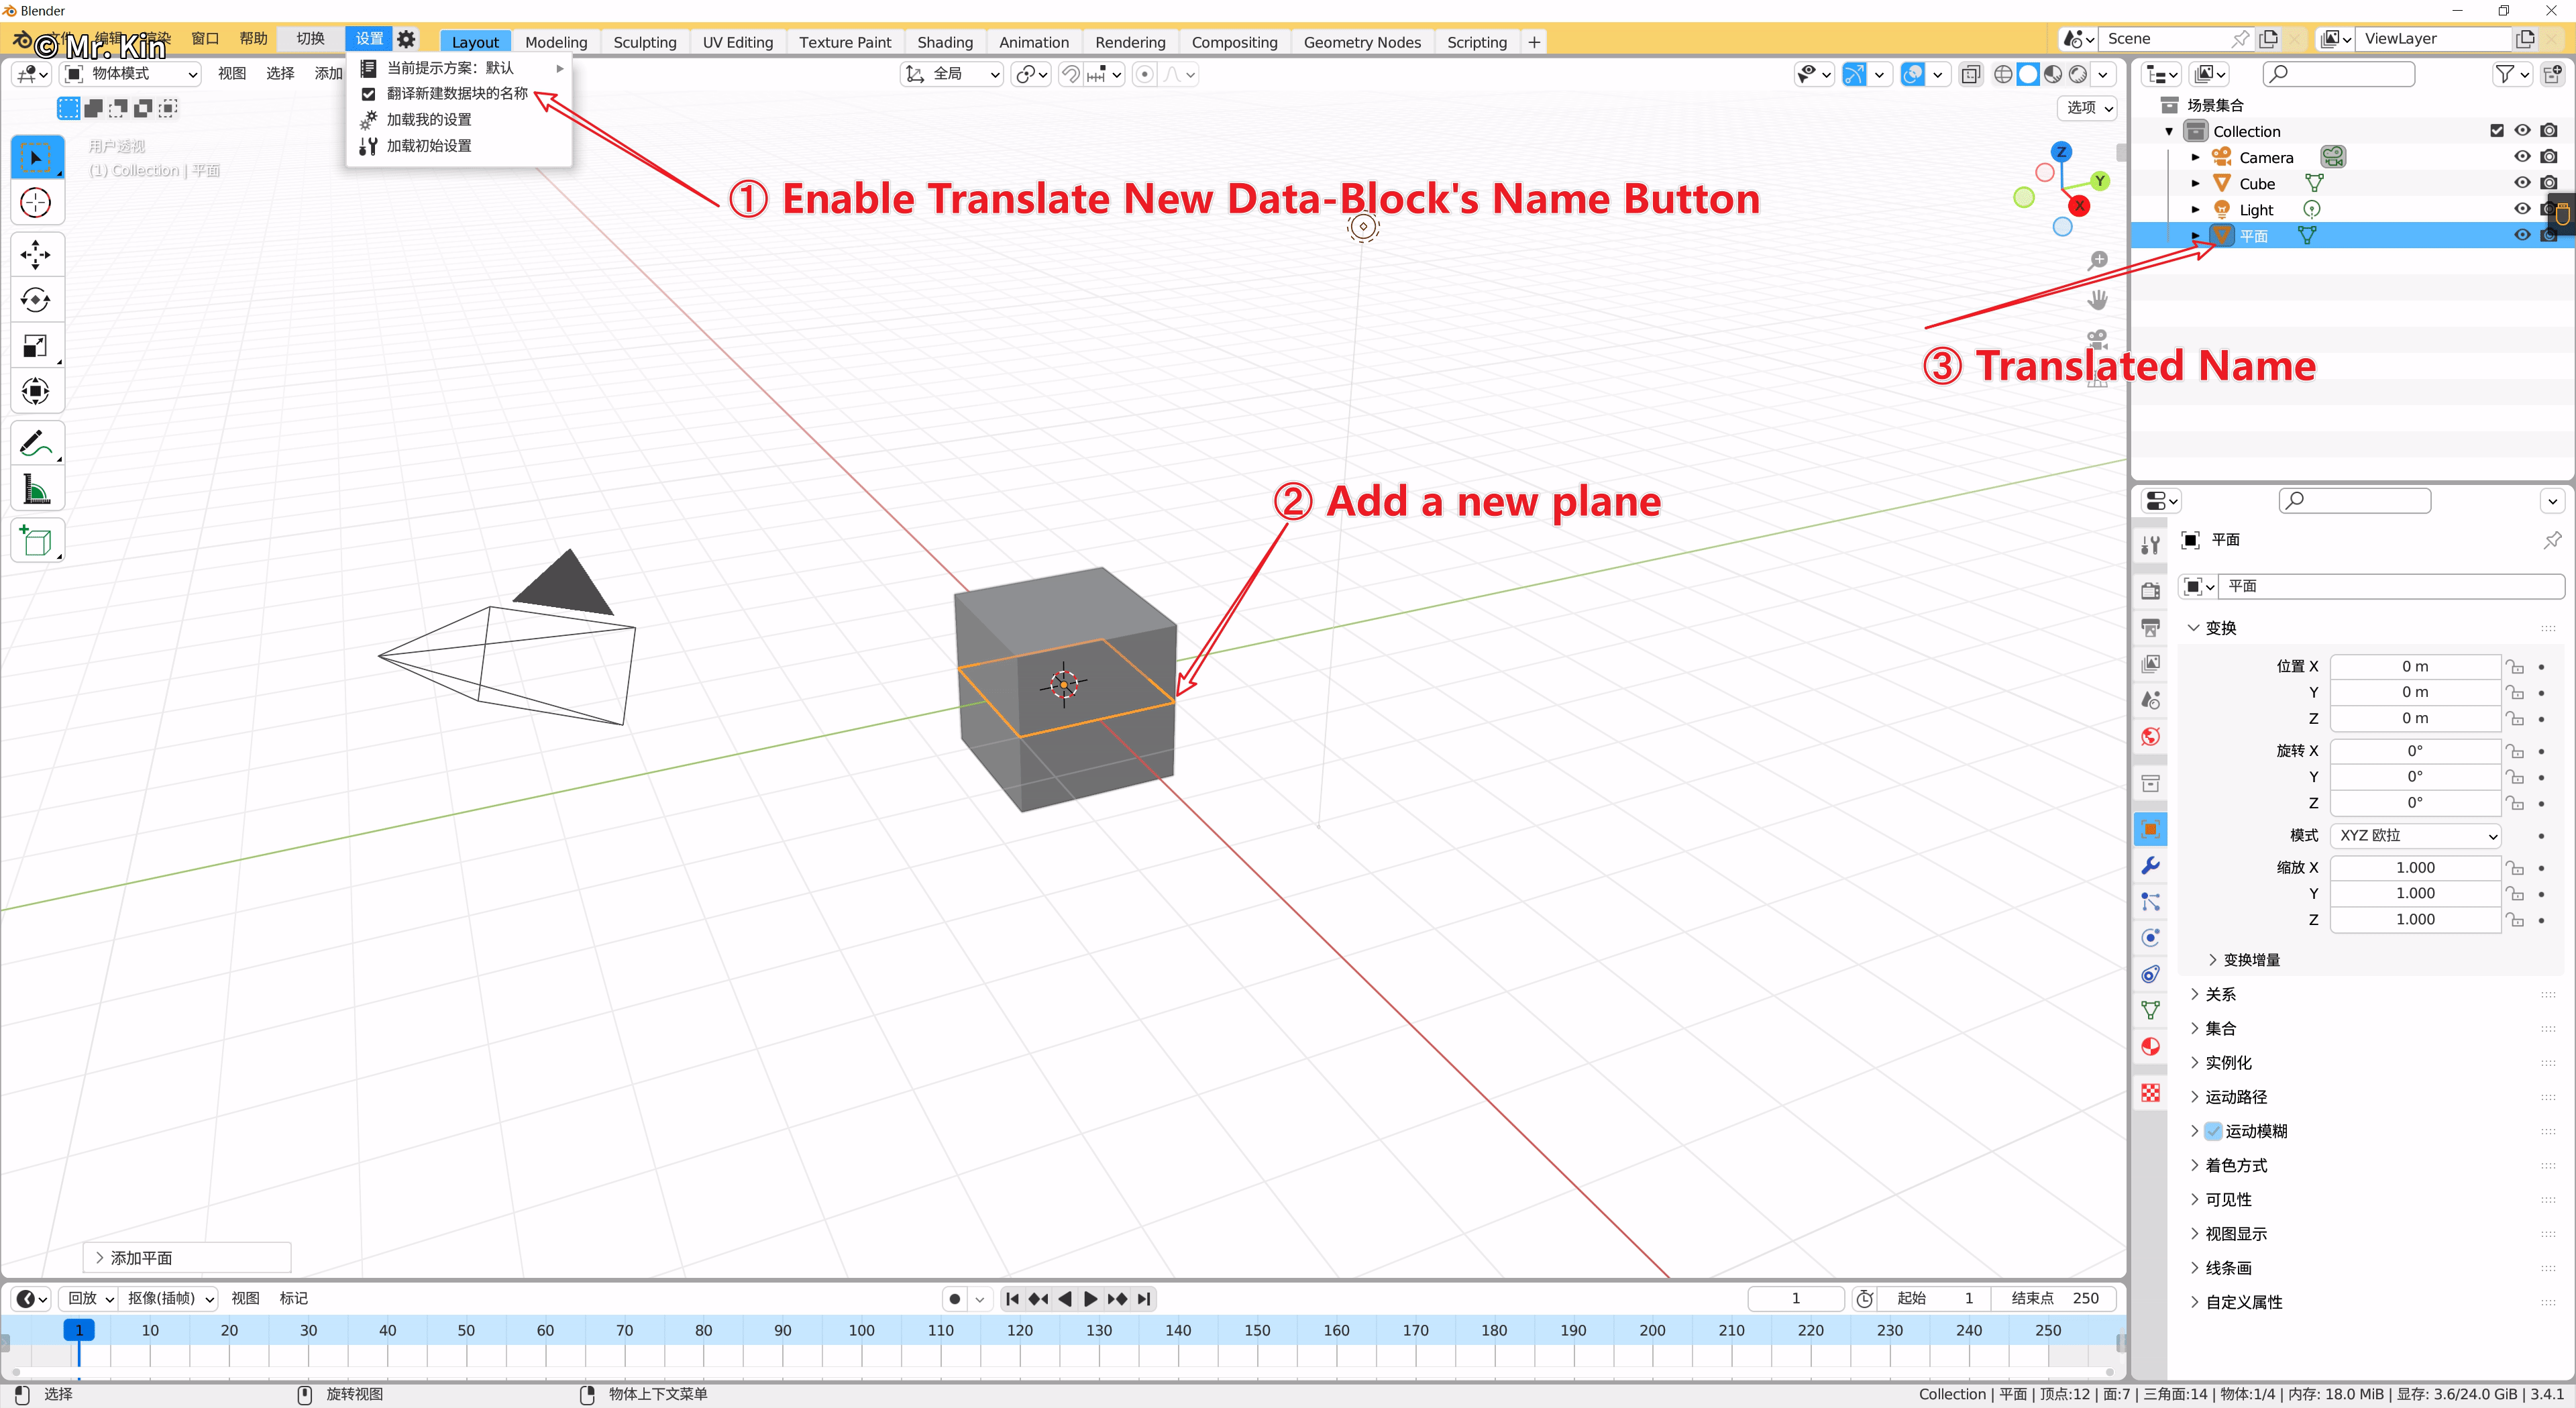
\includegraphics[width=\linewidth]{translate_name_option_effect}
    \caption{翻译新建数据块名称的效果(图示界面语言为简中)}
    \label{翻译名称的效果}
\end{figure}

\subsubsection{插件的键位映射}
\hypertarget{AddonKeymaps}{}
本插件的偏好设置面板中,允许修改插件的键位映射,设置方法和Blender原生的键位映射设置方法一样,如图\myref{插件的键位映射功能}所示。修改键位映射后,均会自动保存相应修改。

\begin{figure}[h!]
    \centering
    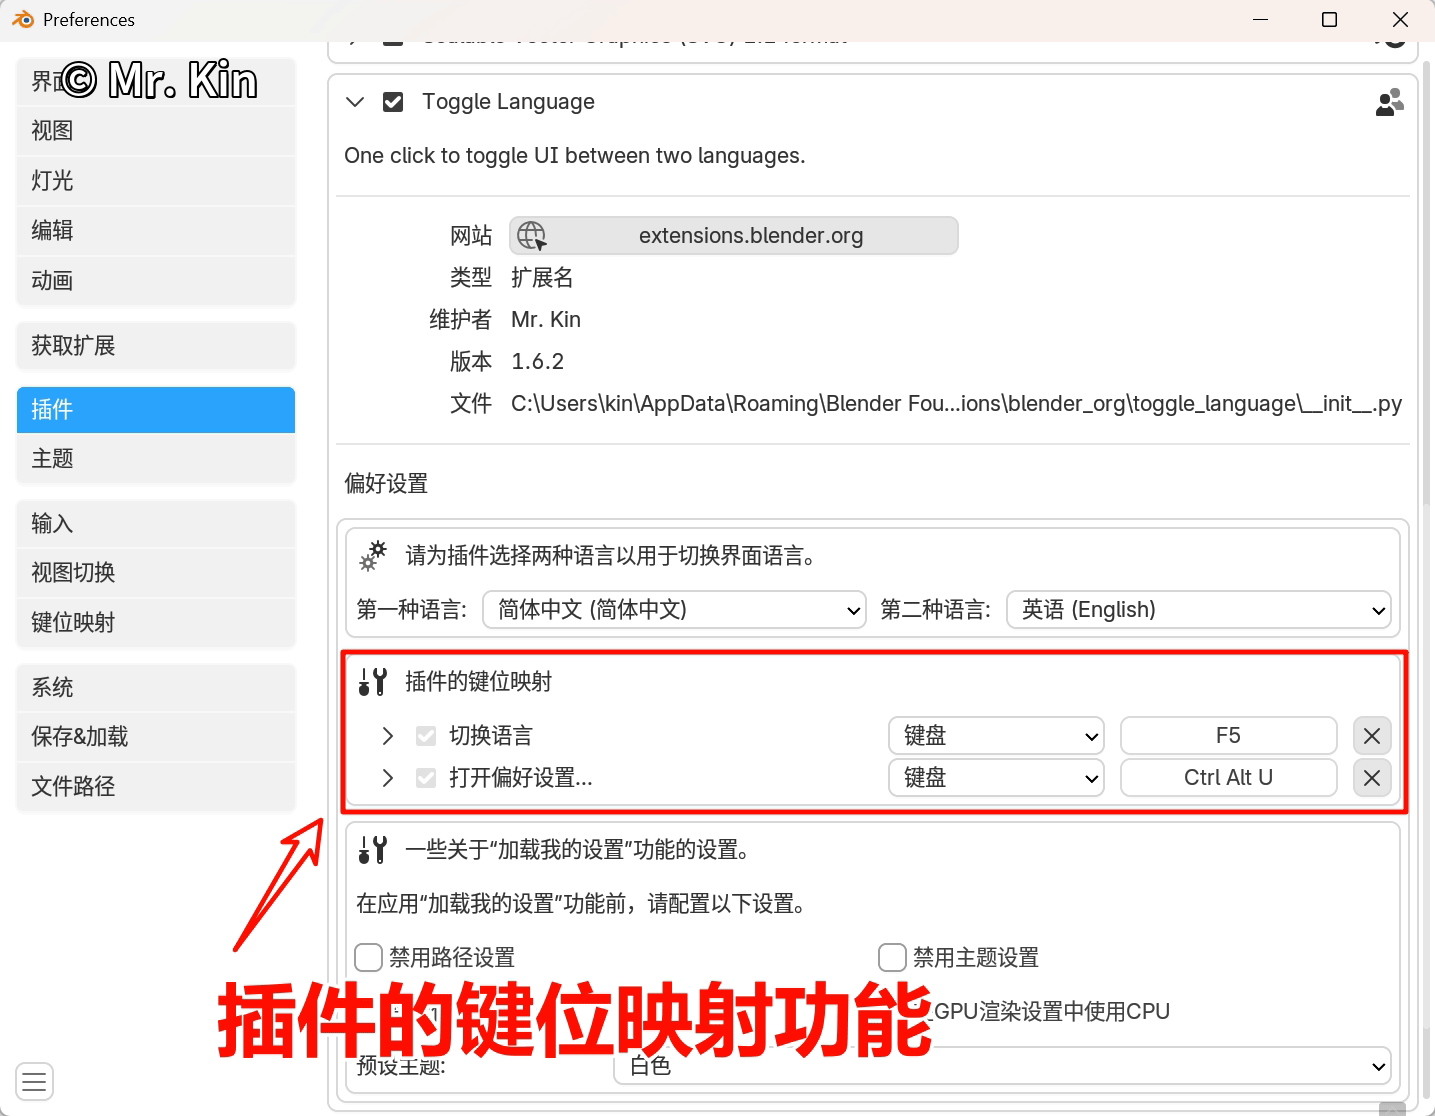
\includegraphics[width=0.8\linewidth]{addon_keymaps}
    \caption{插件的键位映射功能}
    \label{插件的键位映射功能}
\end{figure}

\subsubsection{我的Blender设置(我本人的一些blender设置参数)}
\hypertarget{MySettings}{}
开发这个功能主要是为了方便我一键设置恢复个人的偏好设置,比如更换设备使用blender时,通过下载安装本插件就可以一键恢复设置,而无需拷贝配置文件。

详细的设置参数情况如下:
\begin{enumerate}
    \item 偏好设置部分:
    \begin{enumerate}
        \item 界面>分辨率缩放到1.3
        \item 界面>编辑器>状态栏>启用「场景统计数据」「系统内存」「显存」(v2.90以上版本才有)
        \item 主题> White
        \item 插件>启用插件Node Wrangler、Cell Fracture、Auto Tile Size、Development: Icon Viewer(v3.0以上版本的不含有Auto Tile Size插件)
        \item 视图切换>启用「围绕选择物体选择」和「缩放至鼠标位置」
        \item 键位映射>启用「Pie Menu on Drag」和「Extra Shading Pie Menu Items」
        \item 系统
        \begin{enumerate}
            \item Cycles渲染设备> 有显卡设备时会自动选择启用显卡设备,无显卡时设置为默认NONE(当检测到英伟达显卡时,若OPTIX可用时则优先选择。默认下仅启用显卡,不含CPU,若需要CPU和GPU混合渲染,请在\hyperlink{加载我的设置小节}{加载我的设置的设置参数}中开启)
            \item 内存和限额>撤销次数>256
            \item 声音>音频设备> SDL(v2.83版本才有)
        \end{enumerate}
        \item 保存\&加载>启用「压缩文件」
        \item 文件路径
        \begin{enumerate}
            \item 纹理:H:/textures/
            \item 渲染输出:D:/process/
        \end{enumerate}
    \end{enumerate}
    \item 启动文件部分(注意:使用「我的设置」功能,会同时将以下设置保存进启动文件):
    \begin{enumerate}
        \item 属性编辑器
        \begin{enumerate}
            \item 渲染属性
            \begin{enumerate}
                \item 渲染引擎> Cycles
                \item 设备> GPU计算(有GPU设备时会自动启用,无显卡则设置为CPU)
                \item 采样>启用「自适应采样」(v2.9之后版本才有,含v2.9。v3.0之后版本默认启用)
                \item 采样>启用「自适应采样」>噪波阈值>0.1
                \item 采样>最大采样>渲染设置为250,视图设置为1
                \item 采样>降噪>通道>反照和法向
                \item 采样>降噪>降噪器(当OPTIX可用时优先选择,v2.9系列版本设置为NLM,其余为OPEN IMAGEDENOISE,v2.83是自带的其他降噪方法)
                \item 采样>降噪>降噪器>OpenImageDenoise > 使用 GPU(v4.1 之后版本才有,含 v4.1)
                \item 采样>路径引导(纯CPU渲染才有,v3.4之后版本才有,含v3.4)
                \item 性能> Auto Tile Size > Target Tile Size > 128(v3.0之前版本才有,不含v3.0,v3.0之后版本的不含有Auto Tile Size插件)
                \item 性能 > 内存  > 平铺尺寸 > 4096(v3.0之后版本才有,含v3.0,v3.0之前版本的没有分块渲染功能。设定值为4096是为了避免渲染4k图像时导致分块。)
                \item 性能>线程>多线程模式>固定
                \item 性能>线程>线程> 总线程数量-2(自动检测总线程数量并计算设置,保留两个线程给系统。例如CPU总线程为8,那么插件会设置为6)
                \item 性能>最终渲染>持久数据
            \end{enumerate}
            \item 输出属性>输出路径:D:/process/
        \end{enumerate}
        \item 顶部菜单栏>文件>外部数据>自动打包资源
    \end{enumerate}
\end{enumerate}

考虑到「加载我的设置」功能比较偏个性化,并非适合所有人,所以我专门又开发设计了一些设置值来控制其中部分功能。如果你想用「加载我的设置」功能,但又不喜欢其中所有功能,就可以通过这些设置值来单独控制。这些设置值位于插件偏好设置面板中,如图\myref{加载我的设置的设置参数}所示,首先设置对应参数,再应用「加载我的设置」功能。

关于「加载我的设置」的一些设置参数如下:
\hypertarget{加载我的设置小节}{}
\begin{itemize}
    \item 禁用路径设置:禁用路径参数设置(默认不启用,即设置路径参数)。
    \item 禁用主题设置:禁用主题参数设置(默认不启用,即设置个性化主题)。
    \item 禁止保存启动文件:在应用「加载我的设置」时,禁止保存启动文件,因此所设置的参数不会写入启动文件中(默认不启用,即保存启动文件)。
    \item 在GPU渲染设置中使用CPU:Cycles渲染设备中同时选择CPU(默认不启用,即纯GPU渲染,不含CPU设备。启用后效果是CPU和GPU混合渲染)。
    \item 预设主题:blender主题(默认白色,当启用「禁用主题设置」后,该选项无效)
\end{itemize}

\begin{figure}[h!]
    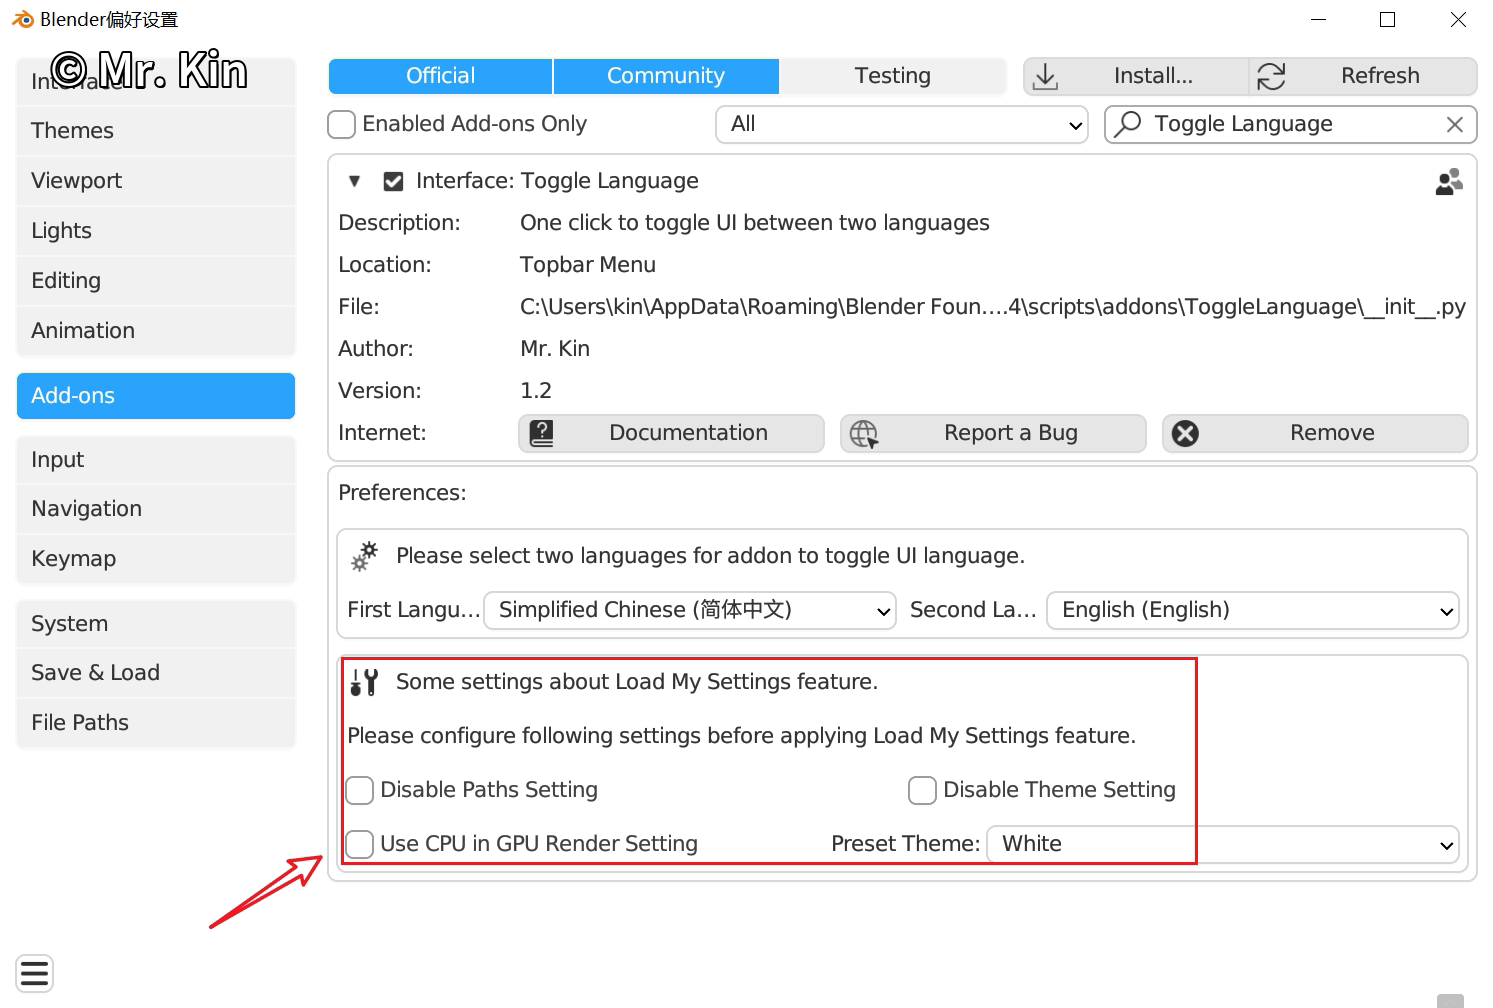
\includegraphics[width=\linewidth]{settings_for_loading_my_settings}
    \caption{关于「加载我的设置」的一些设置参数}
    \label{加载我的设置的设置参数}
\end{figure}

\subsubsection{关于使用翻译新建数据块的名称按钮的说明}
需要注意的是,翻译新建数据块的名称按钮设置值是无法随用户偏好设置自动保存。该功能的代码实现:其 property 属性值是注册在 bpy.types.Scene 中。因此,无法通过用户偏好设置中自动保存设置的功能进行存储。不像本插件偏好设置面板中的两种语言的属性值,后者是通过 bpy.types.AddonPreferences 类实现的,它可以通过用户偏好设置中自动保存设置的功能进行存储\footnote{实际上,在禁用用户偏好设置的自动保存设置功能后,本插件偏好设置面板中的两种语言的属性值也无法自动存储,需要保存在某一工程文件中才行。}。

建议:若需要保存该功能的设置值,请保存一个工程文件\footnote{保存在启动文件也是可行的。}(.blend),该功能的设置值会保存在这个工程文件。

\section{已知问题}
\subsection{加载初始设置按钮导致闪退}
在未保存工程文件\footnote{例如通过安装路径打开主程序的情况或者打开一个工程文件后进行修改却未保存的情况。}(.blend)的情况下,加载初始设置功能会有机率引起异常码EXCEPTION\_ACCESS\_VIOLATION,从而导致blender闪退,目前暂未查明原因。在导致blender闪退时,重置功能的代码执行的不完整,一般是成功地加载初始偏好设置并保存,而初始启动文件并未成功加载并保存。因此,在该功能导致blender闪退后,还请用户自行重置偏好设置及启动文件。

建议:在使用该功能之前,请先保存一个工程文件(.blend)。

\section{开发记录}
\subsection{开发与测试环境}
\begin{itemize}
    \item OS: Win11 v24H2 / Win10 v22H2 / Kali Linux 2021.3 / Mac
    \item Blender: v2.83 ‑ v4.3.2
\end{itemize}

\subsection{更新历史}
表\myref{更新历史}记录了本插件各个版本的更新历史。
\begin{longtable}{|*{2}{c|}m{300pt}|}
    \caption{插件的更新历史}\label{更新历史} \\
    \hline
    版本 & 更新日期 & \multicolumn{1}{c|}{更新内容} \\
    \hline
    \endfirsthead

    \caption{插件的更新历史(续)} \\
    \hline
    版本 & 更新日期 & \multicolumn{1}{c|}{更新内容} \\
    \hline
    \endhead

    \href{https://github.com/Mister-Kin/ToggleLanguage/releases/tag/v1.6.2}{v1.6.2} & 2024-12-15 & 新增功能:插件键位映射;优化:为操作器确认对话框添加更多提示信息;优化:润色部份提示文字……\\
    \hline
    \href{https://github.com/Mister-Kin/ToggleLanguage/releases/tag/v1.6.1}{v1.6.1} & 2024-07-01 & 在blender v4.1中为OpenImageDenoise启用gpu;支持blender v4.2\\
    \hline
    \href{https://github.com/Mister-Kin/ToggleLanguage/releases/tag/v1.6}{v1.6} & 2023-11-19 & 修复并适配blender v4.0 \\
    \hline
    v1.5.1 & 2023/08/23 & 修复:optix\_exist 变量引用前未分配;优化:润色翻译 \\
    \hline
    v1.5 & 2023/04/21 & 新增功能:添加视频进度条;新增功能:添加实用工具菜单…… \\
    \hline
    v1.4 & 2023/04/16 & 新增功能:删除所有集合和物体;新增功能:添加复选框禁用保存启动文件……\\
    \hline
    v1.3.1 & 2023/03/29 & 更新文档链接 \\
    \hline
    v1.3 & 2023/01/24 & 修复:optix\_exist变量引用前未分配;优化降噪设置……\\
    \hline
    v1.2 & 2023/01/15 & 优化「加载我的设置」功能;优化「翻译新建数据块名称」功能…… \\
    \hline
    v1.1 & 2022/10/16 & 修复偏好设置一直被修改导致无法消星的情况;移除 keymaps.py 中的注释代码…… \\
    \hline
    v1.0 & 2022/01/12 & 移除 F6 快捷键的支持;paths 路径统一为小写格式…… \\
    \hline
    v0.9 & 2021/11/06 & 重构:拆分文件规范化开发;加载我的设置功能支持更多的系统和硬件平台……\\
    \hline
    v0.8 & 2021/08/30 & 支持切换更多语言;支持完整翻译插件UI;为某些功能添加交互提示(信息框,确认框等)…… \\
    \hline
    v0.7 & 2021/07/11 & 我的偏好设置支持blender v2.93;重写property代码 \\
    \hline
    v0.6 & 2021/03/10 & 添加布尔值按钮-新数据翻译;支持快捷键;代码重构,插件翻译重构…… \\
    \hline
    v0.5 & 2020/12/08 & 支持blender v2.91;支持从.zip文件安装插件…… \\
    \hline
    v0.5-beta & 2020/09/20 & 添加菜单用以选择UI提示方案 \\
    \hline
    v0.4 & 2020/08/03 & 代码项目重命名为ToggleLanguage;按钮UI放置于最右端;添加新按钮以快速查看preferences \\
    \hline
    v0.3 & 2020/06/05 & 更新至blender 2.83 API;修改部分类名;添加文档链接;修改完善许可说明 \\
    \hline
    v0.2 & 2020/05/21 & 清除未使用属性的报错 \\
    \hline
    v0.1 & 2020/05/12 & 完成基础的功能设计「一键切换」 \\
    \hline
\end{longtable}

\note{更多详细的信息,请查看 \href{https://github.com/Mister-Kin/ToggleLanguage/releases}{Release Notes}。}

\section{作者}
\textbf{ToggleLanguage} © Mr. Kin, 项目代码采用 \href{https://github.com/Mister-Kin/ToggleLanguage/blob/master/LICENSE}{GNU GPL v3.0} 许可协议进行发布。

由 Mr. Kin 著作并维护。

\inputBibliography
\appendix
% 附录

\end{document}
